\documentclass[msc,oneside,a4paper]{udelar}

\lstdefinestyle{customc}{
	belowcaptionskip=1\baselineskip,
	breaklines=true,
	frame=L,
	xleftmargin=\parindent,
	language=C,
	showstringspaces=false,
	basicstyle=\footnotesize\ttfamily,
	keywordstyle=\bfseries\color{green!40!black},
	commentstyle=\itshape\color{purple!40!black},
	identifierstyle=\color{blue},
	stringstyle=\color{orange},
}

\lstdefinestyle{customasm}{
	belowcaptionskip=1\baselineskip,
	frame=L,
	xleftmargin=\parindent,
	language=[x86masm]Assembler,
	basicstyle=\footnotesize\ttfamily,
	commentstyle=\itshape\color{purple!40!black},
}

\lstset{escapechar=@,style=customc}

\pgfplotsset{compat=1.16}

\bibliographystyle{unsrtnat}

% ===== FIN DEL PREÁMBULO =====

% ===== INICIO DEL DOCUMENTO =====

\begin{document}


  \title{Tesis de grado}
  \subtitle{Iluminación global con superficies especulares}
  \institutelogo{1} 
  \institutelogo{2} 
  \author{Bruno}{Sena}
  \escritura{en} 
  
  \director{}{José}{Aguerre}{}
  \director{}{Eduardo}{Fernández}{}
  
  \examiner{}{NombreTribunal1}{ApellidoTribunal1}{}
  \examiner{}{NombreTribunal2}{ApellidoTribunal2}{}
  \examiner{}{NombreTribunal3}{ApellidoTribunal3}{}
  
  \graduatename{Ingeniería en Computación}
  \institute{Facultad de Ingeniería}{FIng}

  \graduatelocation{Montevideo}{Uruguay}
  
  \date{\the\day}{\the\month}{\the\year}


  \keyword{iluminación global}
  \keyword{radiosidad}
  \keyword{reflexión especular}

        
  \maketitle 
    
  \frontmatter 
  \afterpage{\blankpage}
  % !TeX spellcheck = es_ES
\begin{abstract}

Los algoritmos de iluminación global simulan el comportamiento de la luz en la naturaleza. La síntesis de imágenes fotorealistas generadas por computadora o la evaluación del diseño lumínico para arquitectura son algunos de los objetivos abarcados por este tipo de algoritmo.

En este contexto, este proyecto se enmarca en el estudio, análisis y adaptación de técnicas que proponen extensiones a el método de radiosidad. Este método se basa en el estudio de la transferencia de energía lumínica entre superficies que componen una escena. Para simplificar el cálculo del intercambio de radiación entre elementos de la escena es subdividida en una cantidad de superficies planas discreta, que se denominan parches.

Este método de radiosidad clásico considera únicamente superficies lambertianas, es decir, reflectores difusos perfectos. Esta limitación supone que el método no pueda aplicarse en una gran variedad de escenas donde la incidencia de la reflexión especular tiene una gran incidencia en la iluminación de la escena.\footnote{Disponible en GitHub: https://github.com/brunosegiu/radiosum}.

La extensión planteada propone la construcción de un algoritmo capaz de considerar superficies especulares. Por otro lado, se proponen técnicas que permitan proveer nuevos acercamientos al cálculo de los factores de forma utilizando técnicas de paralelismo para el hardware moderno.

\end{abstract}

  \tableofcontents          
  \afterpage{\blankpage}  
 
  \mainmatter

  \afterpage{\blankpage} 
  % !TeX spellcheck = es_ES
\chapter{Introducción}
\label{ch:chap01}

%================================================================================================
% Introducción 
%================================================================================================


%================================================================================================
% Motivación y problema
%================================================================================================

\section{Motivación y problema}
\label{sec:motivacionYProblemas}

Naturalmente, el fenómeno de la iluminación ocurre cuando una fuente luminosa emite un conjunto flujo de fotones, normalmente conocido como rayo o haz de luz, que recorre un camino hasta intersectar una superficie que lo bloquee. Según la óptica, los fenómenos que pueden manifestarse debido a esta interacción son la \textit{absorción, reflexión, refracción o fluorescencia}; pues una superficie puede conservar parte de la energía transmitida afectando el color percibido, reflejarla en distintas direcciones, modificar la dirección del haz al poseer propiedades de transparencia o re-emitir la energía de forma fluorescente en alguna dirección particular.

Estas interacciones observadas son de gran interés para la computación gráfica, dado que su estudio tiene gran relevancia en la arquitectura y la industria del entretenimiento. En particular, la generación de modelos capaces de simular el transporte de la luz en espacios tridimensionales es uno de los mayores motivadores de los avances en computación gráfica. A lo largo del siglo $XX$ y $XXI$ se han propuesto distintos modelos (\cite{Kajiya}, \cite{Cohen}) que aproximan el comportamiento real de la luz en distintos entornos con variados niveles de foto-realismo y desempeño.

Históricamente, se destacan tres acercamientos al cálculo de la iluminación. La traza de rayos, el método de radiosidad y el mapeado de fotones. Estas técnicas se concibieron con un motivo similar, la construcción de algoritmos que emulen la iluminación indirecta, es decir, los caminos de iluminación de la forma \textbf{L(S|D)*E} (estos son los caminos trazados por un haz de luz que parte de la fuente luminosa, interseca superficies especulares o difusas y llega al punto de vista del observador). 

Si bien las técnicas consideradas tienen el potencial de resolver estos caminos el método de radiosidad tiene la capacidad de resolver los caminos de la forma \textbf{LD*E} (únicamente se considera el fenómeno de la reflexión difusa) de forma eficiente a través del modelado de el fenómeno de la iluminación como el transporte de energía térmica entre superficies. Mientras que la traza de rayos y mapeado de fotones ponen especial énfasis en los caminos \textbf{LS*DE}, pues considerará con mayor importancia las reflexiones especulares.

El avance del \textit{hardware} introducido en los últimos años significa que es necesario re-evaluar técnicas y algoritmos constantemente, con el objetivo de generar algoritmos que provean resultados foto-realistas en tiempos de ejecución mínimos. Si bien en los últimos años se han desarrollado las técnicas de \textit{trazado de rayos bi-direccional} y otras técnicas de \textit{trazado de rayos de Monte Carlo} con el objetivo de atacar el problema de la reflexión difusa utilizando el algoritmo de traza de rayos. No obstante, también se han propuesto variantes que extienden los métodos de radiosidad para considerar los efectos introducidos por las superficies especulares.

%================================================================================================
% Objetivos
%================================================================================================

\section{Objetivos}
\label{sec:objetivos}

Este proyecto tiene el objetivo de \textbf{analizar} las técnicas de extensión del método de radiosidad a caminos de la forma \textbf{L(S|D)*E}, generando \textbf{adaptaciones} de las extensiones propuestas por la Academia a un conjunto de técnicas establecidas en la Industria, generando la \textbf{implementación} correspondiente a los distintos algoritmos formulados con la finalidad de \textbf{comparar} cualitativamente el rendimiento computacional observado en \textit{hardware} moderno así como el error introducido por las aproximaciones que se consideran al discretizar el problema concebido.

En este sentido, se explorarán tres alternativas para el cálculo de la radiosidad entre las superficies que componen la escena virtual considerada; aprovechando la implementación eficiente en \textit{hardware} de un conjunto de funcionalidades que facilitan la proyección de gráficos tridimensionales así como el uso de recursos eficiente a través del paralelismo.  

%================================================================================================
% Estructura el documento
%================================================================================================

\section{Estructura del documento}
\label{sec:estructuraDelDocumento}

El resto del documento se estructura de la siguiente manera. El Capítulo 2 introduce el estado del arte en técnicas de iluminación global, con especial énfasis en la técnica de radiosidad y sus extensiones; además, se exploran diversos acercamientos alternativos al problema a resolver. El Capítulo 3 refiere al diseño de la solución que se ha propuesto para resolver y facilitar la construcción de pruebas de los algoritmos implementados. El Capítulo 4 contiene detalles de implementación, detallando distintas decisiones tomadas para eludir un conjunto de obstáculos técnicos observados. En el Capítulo 5, se encuentra una síntesis de los casos de prueba considerados así como los un análisis de los resultados obtenidos junto a un conjunto de ventajas y desventajas que se han observado. Finalmente, se proveen un conjunto de conclusiones y posible trabajo a futuro detectado a lo largo de la construcción del proyecto.
  % !TeX spellcheck = es_ES
\chapter{Estado del arte}
\label{ch:chap02}

Este capítulo introduce un resumen de las áreas más importantes relacionadas al trabajo realizado en este proyecto, incluyendo los modelos de iluminación por computadora, el método de radiosidad y sus posibles implementaciones y extensiones.

\section{Modelos de iluminación}
\label{sec:dibujado}

El proceso de dibujado de gráficos tridimiensionales por computadora comprende la generación automática de imágenes con cierto nivel de realismo a partir de modelos que componen una \textit{escena} o \textit{mundo} tridimencional, junto a un conjunto de cualidades físicas que rigen las formas en la que la luz interactúa con los objetos.

Este problema puede ser reducido al problema de cálculo del valor de intensidad lumínica observada en un punto $x$ y proveniente directamente de un conjunto de puntos, representado por $x'$. En  \citeyear{Kajiya}, \citeauthor{Kajiya} presentó uno de los modelos más aceptado por la comunidad por su generalidad, la denominada <<ecuación del \textit{rendering}>>:

\begin{equation}
    I(x,x') = g(x,x') \bigg[\epsilon(x,x') + \int_{S} \rho(x,x',x'')I(x',x'') \delta x''\bigg] \label{eq:rendering}
\end{equation}
donde:
\begin{itemize}
    \item $I(x,x')$ describe la intensidad lumínica que llega al punto $x$ proveniente de $x'$
    \item $g(x,x')$ es un término geométrico, toma el valor de $0$ si existe oclusión entre $x'$ y $x$, y en otro caso su valor es $\dfrac{1}{r^{2}}$ donde $r$ es la distancia entre ambos puntos.
    \item $\epsilon(x,x')$ expresa la intensidad lumínica emitida por la superficie en el punto $x'$ en dirección a $x$
    \item $\int_{S} \rho(x,x',x'')I(x',x'') \delta x''$ está compuesta por dos términos:
        \begin{itemize}
            \item $\rho(x,x',x'')$ es el término de reflectividad bi-direccional, es decir la proporción de luz que va desde $x''$ a $x$ pasando por $x'$
            \item $I(x',x'')$ describe la intensidad lumínica observada en el punto $x'$ proveniente de $x''$
        \end{itemize}
    por lo que este término refiere a la intensidad percibida desde $x$ considerando todas las reflexiones de
    luz posibles para el dominio $S$.
\end{itemize}

Existen distintos métodos de resolución de la ecuación del rendering, donde la la mayoría implican cálculos aproximados dado el gran costo de cómputo requerido para hallar su valor preciso. Estos métodos balancean el costo computacional de los algoritmos utilizados y el error del valor obtenido. Existen dos categorías principales para el método: \textit{local} y \textit{global}. Un ejemplo de ambos modelos puede ser observado en la Figura \ref{local-vs-global-img}.

\vspace{5mm}
\begin{figure}[h]
	\begin{subfigure}{0.5\textwidth}
		  	\centering
   		 	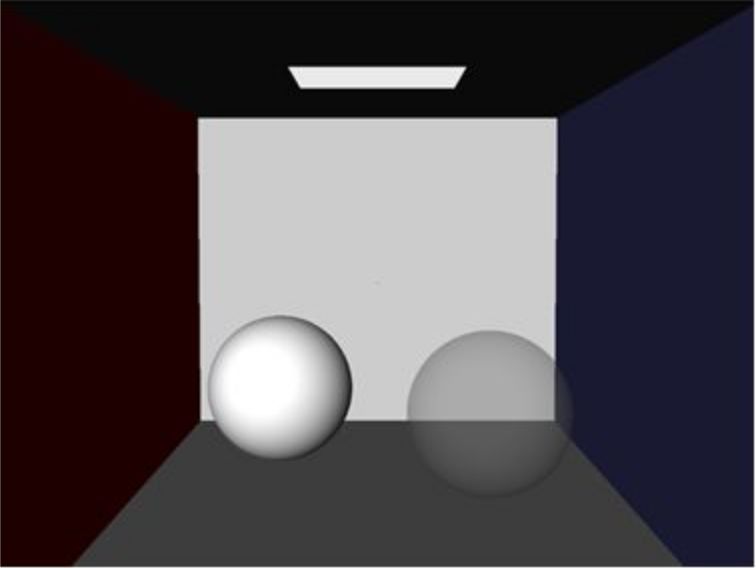
\includegraphics[width=1\linewidth]{assets/local}
   		 	\caption{Local}
   	\end{subfigure}
    \begin{subfigure}{0.5\textwidth}
    	\centering
    	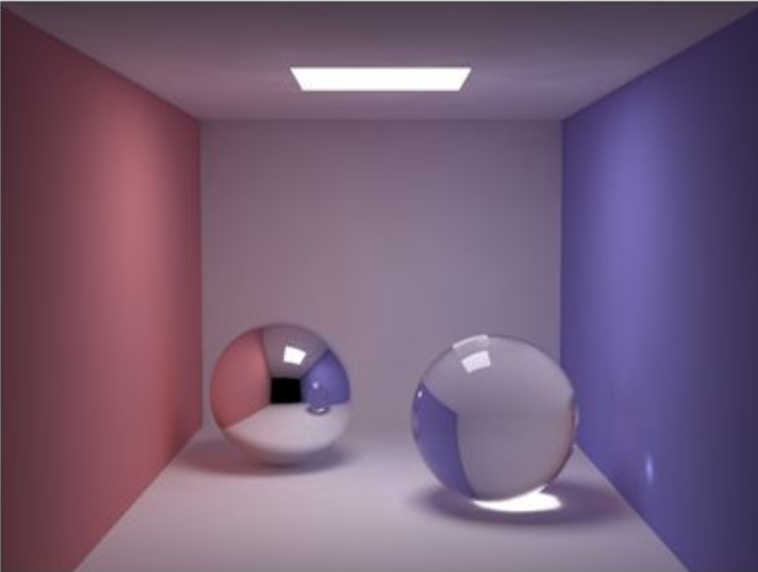
\includegraphics[width=1\linewidth]{assets/global}
    	\caption{Global}
    \end{subfigure}
    \caption{Dibujado utilizando distintos modelos de iluminación.}
    \label{local-vs-global-img}
\end{figure}

\subsection{Iluminación Local}
\label{sec:ilumlocal}
Los modelos de iluminación local tienen en cuenta las propiedades físicas de los materiales
y las superficies de forma individual. Es decir, al dibujar cada objeto no se toman en cuenta las posibles interacciones de los haces de luz con los objetos restantes en la escena. Esto implica que no se proyectan sombras, y tampoco se modelan correctamente las cáusticas producidas por la acumulación de la luz ni el sangrado, entre otros fenómenos de la naturaleza. Estos métodos sencillos de implementar y son frecuentemente utilizados en problemas cuya resolución debe ser realizada en tiempo real o por decisiones artísticas.

En referencia a la ecuación del rendering, el término geométrico nunca toma el valor 0, es decir, no se toma en cuenta las colisiones de la luz con otros objetos. El término $\epsilon(x,x')$ toma un valor constante únicamente dependiente de $x$ y $\int_{S} \rho(x,x',x'')I(x',x'') \delta x''$ toma el valor constante $0$.

\subsection{Iluminación Global}
\label{sec:ilumglobal}

El modelo de iluminación global refiere a un conjunto de técnicas que simulan parcial o completamente las interacciones de la luz con todos los objetos que se encuentran  en la escena. Es decir, en contraposición a la iluminación local, se consideran los fenómenos de reflexión y refracción de la luz.

Dependiendo de las característica de los modelos y algoritmos empleados, pueden obtenerse resultados fotorealistas para diferentes escenarios.

El algoritmo de \textit{path-tracing} emula completamente cada haz de luz desde su incepción en una fuente luminosa siguiendo el camino de interacciones del rayo con las distintas superficies de la escena. En este caso el grado de granularidad (que depende directamente de la cantidad de muestras utilizadas) influye en la precisión y calidad en la imagen final.

Por otro lado, el algoritmo de \textit{mapeado de fotones} simula los efectos producidos por las colisiones de las partículas que componen la luz (fotones) con los objetos, que dejan impresiones que afectarán el resultado final de la imagen.

Existen además distintas variaciones e híbridos de estos métodos ya que los mismos son demasiado costosos como para dibujar imágenes en tiempo real, en sus versiones originales.

\section{Radiosidad}
\label{sec:radiosidad}

El método de radiosidad es una técnica de iluminación global que emula el transporte de la luz entre superficies difusas. El mismo nombre se utiliza también para describir la magnitud física definida como radiosidad, que indica el flujo de energía radiada por unidad de área ($\frac{W}{m^{2}}$).

Originalmente, este modelo de iluminación global fue propuesto por [\citeauthor{Goral}], y se basa en modelos matemáticos similares a los que resuelven el problema de la transferencia de calor en sistemas cerrados dicretos como diferencias finitas o elementos finitos.

\subsection{Radiosidad en superficies lambertianas}

La solución propuesta por \citeauthor{Goral} implica que todas las superficies son idealmente difusas, también conocidas como lambertianas. Estas superficies se comportan como reflectores difusos ideales, lo que significa que reflejan la energía incidente de forma isotrópica siguiendo la regla del coseno como se observa en la Figura \ref{img:lamber}.

\vspace{5mm}
\begin{figure}[h]
	\centering
	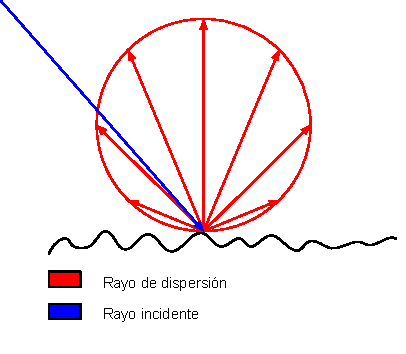
\includegraphics[width=.5\linewidth]{assets/lambert}
	\caption{Reflector lambertiano}
	\label{img:lamber}
\end{figure}

Adicionalmente, se considerará que la energía lumínica irradiada en todas direcciones por cada diferencial de área $\delta_{A}$, puede ser definida como:

\begin{equation}
    I = \frac{\delta{P}}{\cos{\phi\delta\omega}} \label{eq:i}
\end{equation}
donde:
\begin{itemize}
	\item $\omega$ es la dirección de vista.
    \item $I$ es la intensidad de la radiación para un punto de vista particular.
    \item $\delta{P}$ es lae energía de la radiación que emana la superficie en la dirección $\phi$ con ángulo sólido $\delta\omega$.
\end{itemize}

En superficies perfectamente lambertianas, la energía reflejada puede ser expresada como: $\frac{\delta{P}}{\delta{\omega}} = k\cos{\phi}$. Donde $k$ es una constante.
Sustituyendo en \eqref{eq:i} se obtiene: $\frac{\delta{P}}{\delta{\omega}} = \frac{k\cos{\phi}}{\cos{\phi}} = k$, esto implica que la energía percibida de un punto $x$ 
es constante, independientemente del punto de vista.

Es por esto que la energía total que deja una superficie ($P$) puede ser calculada integrando la energía que deja la superficie en cada dirección posible, esto es, se integra la energía saliente en un hemi-esfera centrada en el punto estudiado:

\begin{equation}
    P = \int_{2\pi} \delta{P} = \int_{2\pi} I\cos{\phi}\delta{\omega} = I \int_{2\pi} \cos{\phi}\delta{\omega} = I\pi
    \label{eq:P}
\end{equation}

Por tanto, dada una superficie $S_{i}$, es posible calcular la energía lumínica que deja la superficie utilizando \eqref{eq:P}. Para ello, se discretizan las superficies en parches difusos, lo que transforma la Eq. \eqref{eq:P} en:

\begin{equation}
    B_{i} = E_{i} + \rho_{i} \sum_{j=1}^{N} B_{j} F_{ij} \label{eq:radiosity}
\end{equation}
donde:
\begin{itemize}
    \item $B_{i}$ es la intensidad lumínica (radiosidad) que deja la superficie $i$.
    \item $E_{i}$ es la intensidad lumínica directamente emitida por $i$.
    \item $\rho_{i}$ es la reflectividad del material para la superficie $i$.
    \item $F_{ij}$ se denomina \textit{factor de forma}, un término que representa la fracción de energía lumínica va del parche $i$ al parche $j$. 
\end{itemize}

Cabe destacar que la naturaleza recursiva de la ecuación anterior (para calcular $B_{i}$ se debe conocer $B_{i}$) implica que se toman en cuenta todas las reflexiones difusas que existan en la escena. Como se puede observar, resolver el sistema de $N$ ecuaciones lineales bastaría para conocer la energía emitida por cada parche. 

Los factores de emisión y reflexión, para cada parche $i$: $E_{i}$ y $\mathbf{\rho_{i}}$ respectivamente, dependen de los materiales que compongan la escena y son parámetros dados. Sólo resta computar la matriz de factores de forma $\mathbf{F}$ para poder calcular el vector de radiosidades $B$. 

Para determinar una entrada de la matriz $F_{ij}$ involucrando a las superficies $i$ y $j$ de área $A(i)$, $A(j)$, considerando los diferenciales infinitesimales de área $\delta{A_{i}}$, $\delta{A_{j}}$, representados en la Figura \ref{img:ff2}, el ángulo sólido visto por $\delta{A_{i}}$ es $\delta{\omega} = \frac{\cos{\phi_{j}\delta{A_{j}}}}{r^{2}}$. Sustituyendo en \eqref{eq:P} se obtiene:

\begin{equation}
    \delta{P}_{i}\delta{A_{i}} = I_{i} \cos{\phi_{i}}\delta{\omega}\delta{A_{i}} = \frac{P_{i}\cos{\phi_{i}}\cos{\phi_{j}}\delta{A_{i}}\delta{A_{j}}}{\pi r^{2}}
\end{equation}

\vspace{5mm}
\begin{figure}[h]
	\centering
	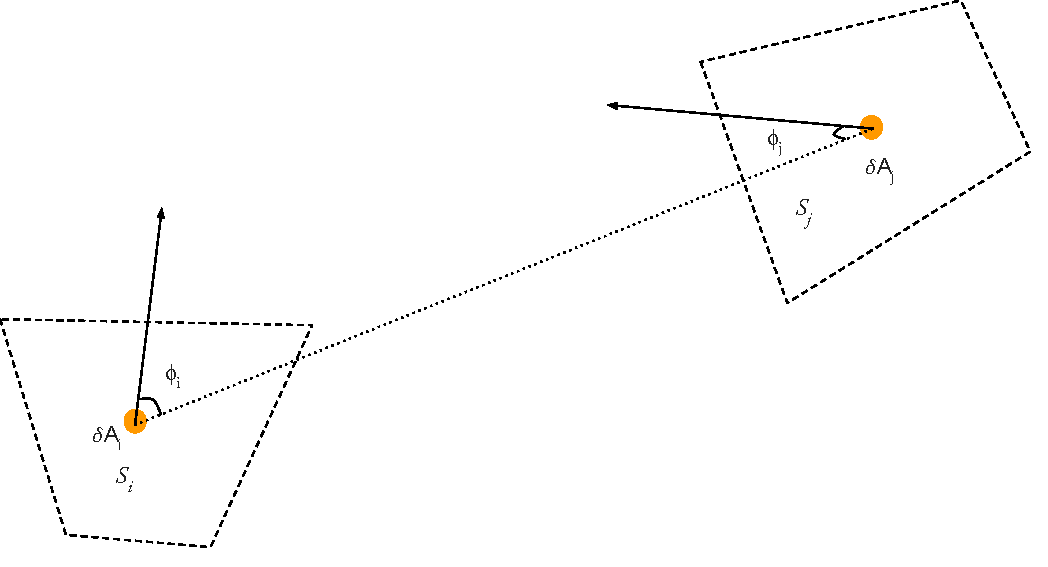
\includegraphics[width=0.8\linewidth]{assets/ff}
	\caption{El factor de forma entre dos superficies}
	\label{img:ff2}
\end{figure}


Considerando que ${P}_{i}{A_{i}}$ es la energía que deja $i$, y que el factor de forma $F_{ij}$ representa la fracción de dicha energía que llega a $j$ podemos observar que:

\begin{equation}
    F_{\delta{A_{i}}-\delta{A_{j}}} = \frac{\cos{\phi_{i}}\cos{\phi_{j}}\delta{A_{j}}}{\pi r^{2}} = \frac{\cos{\phi_{i}}\cos{\phi_{j}}\delta{A_{i}}}{\pi{r^{2}}}
\end{equation}

Integrando, para obtener el factor de forma para el área total:

\begin{equation}
    F_{ij} = \frac{1}{A_{i}} \int_{A_{i}}\int_{A_{j}}\frac{\cos{\phi_{i}}\cos{\phi_{j}}\delta{A_{i}}\delta{A_{j}}}{\pi{r^{2}}} \label{eq:ff}    
\end{equation}

De \eqref{eq:ff} se obtienen las siguientes propiedades:
\begin{enumerate}
	\label{propsff}
    \item $A_{i}F_{ij} = A_{j}F{ij}$, lo que supone una relación simétrica entre los factores de forma.
    \item $\sum_{j=1}^{N} F_{ij} < 1$ Es decir, la suma de una de las filas de la matriz de factores de forma no podrá tener un valor superior a la unidad.
    \item $F_{ii} = 0$ Esto se debe a que los parches considerados son planos y por tanto no reflejan su propia luz.
    \item $F_{ij}$ toma el valor correspondiente a la proyección de $j$ en una hemiesfera unitaria centrada en $i$, proyectándola a su vez en un disco unitario.
\end{enumerate}


\section{Métodos de cálculo de la matriz de Factores de Forma}
\label{sec:calculoff}

El cálculo de los factores de forma a través de la Eq. \eqref{eq:ff} analíticamente es inviable en la práctica pues supone la necesidad de conocer la visibilidad entre cada par de parches que componen la escana. Por tanto, es necesario establecer otros métodos que provean aproximaciones lo suficientemente correctas.

Geométricamente, puese establecerse una analogía para la computación de factores de forma conocida como <<analogía de Nusselt>> (ver Figura \ref{img:nusselt}). Se expresará el factor de forma como la proporción de área proyectada de $S_{j}$ en una hemi-esfera ubicada en el baricentro de $S_{i}$ y luego en un disco centrado en $S_{i}$.

\begin{figure}[H]
	\centering
	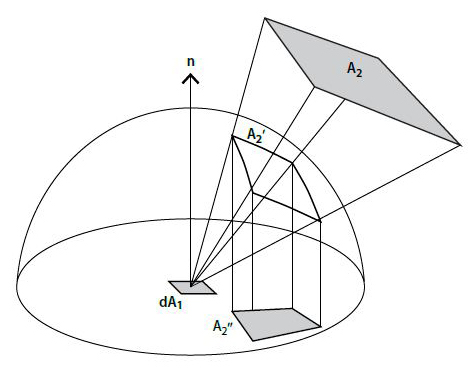
\includegraphics[width=0.55\linewidth]{assets/nusselt}
	\captionof{figure}{La analogía de Nusslet}
	\label{img:nusselt}
\end{figure}

El cálculo de la matriz de factores de forma $\mathbf{F}$ supone la proyección de los parches. De aquí en más se asumirá que estos parches son polígonos no curvos y lo que permite utilizar las técnicas de dibujado de objetos tridimensionales tradicionales.

\subsection{Rasterización}
\label{sec:rasterizacion}

El <<\textit{rendering pipeline}>> es un proceso de dibujado estandarizado que consiste en un conjunto de etapas cuyo cometido es la generación de un \textit{frame buffer}. Los fabricantes de los dispositivos aceleradores gráficos y/o sistemas operativos proveen de interfaces de programación (OpenGL, Vulkan, DirectX) que se basan en este modelo para abstraer el uso del hardware.

Si bien el <<\textit{rendering pipeline}>> es modificable, cada una de sus etapas están definidas.  El programador es capaz de modificar pequeñas funciones (también llamadas \textit{kernels} o \textit{shaders}) que son ejecutadas en la GPU en las etapas correspondientes. El cometido de estas funciones es procesar los parámetros de entrada para generar parámetros que recibirá la siguiente etapa, que los recibirá y transformará como corresponda.

A continuación, se describe el proceso para OpenGL 4.5 visualizado en la Figura \ref{img:pipelinegl}, aunque muchas de estas etapas son trasladables a otras tecnologías existentes.

\begin{enumerate}
	\item Procesamiento de primitivas geométricas:
		\begin{enumerate}
			\item Especificación de vértices: Inicialmente, las aplicaciones indican un conjunto de vértices a dibujar, definiendo cierto conjunto de primitivas geométricas como triángulos, cuadriláteros, puntos, líneas u otros.
			\item \textit{Vertex shader}: Esta etapa transforma los vértices de entrada suministrados por la aplicación. Generalmente se computan las transformaciones lineales necesarias para cambiar la base de las coordenadas de los vértices de un sistema local al sistema global que defina la aplicación. Las coordenadas retornadas deberán corresponderse con coordenadas del espacio de recorte. Es decir, coordenadas correspondientes al volumen de vista.
			\item Teselado: En esta etapa se procesan los vértices a nivel de primitiva geométrica, con el objetivo de subdividirlas para mejorar la resolución obtenida.
			\item \textit{Geometry shader}: En esta etapa también se procesan los vértices a nivel de primitiva geométrica con el objetivo de mutarlas y replicarlas.
			\item Recortado: Esta etapa es \textit{fija}, es decir, no es programable. Todas las primitivas calculadas anteriormente que residan fuera del volumen de vista serán descartadas en las etapas futuras. Además, se transforma las primitivas a coordenadas de espacio de ventana.
			\item Descarte: El proceso de descarte (en inglés \textit{culling}), es también fijo. Consiste en la eliminación de primitivas que no cumplan ciertas condiciones, como por ejemplo el descarte de caras cuya normal tiene dirección opuesta a la del observador.
		\end{enumerate}
	\item Procesamiento de fragmentos (rasterización):
		\begin{enumerate}
			\item Rasterización: El proceso de rasterización discretiza las pirmitivas en espacio de pantalla en un conjunto de fragmentos.
			\item \textit{Shader de fragmentos}: El procesamiento de cada fragmento se realiza a través del \textit{shader de fragmentos} que calcula uno o más colores, un valor de profundidad, y valores de plantilla (del inglés \textit{stencil}).
			\item \textit{Scissor test}: Todos los fragmentos fuera de un área rectangular definida por la aplicación son descartados.
			\item \textit{Stencil test}: Los fragmentos que no pasan la función de planilla definida por la aplicación no son dibujados, por ejemplo, simular el \textit{scissor test} que requieran primitivas más complejas.
			\item \textit{Depth test}: En esta etapa se ejecuta el algoritmo del Z-Buffer, donde sólo se escribirá el resultado en el \textit{frame buffer} de aquellos fragmentos que tengan la menor profundidad. Es decir, los que se encuentren más cerca del observador.
		\end{enumerate}
\end{enumerate}

\clearpage

\vspace{5mm}
\begin{figure}[H]
	\centering
	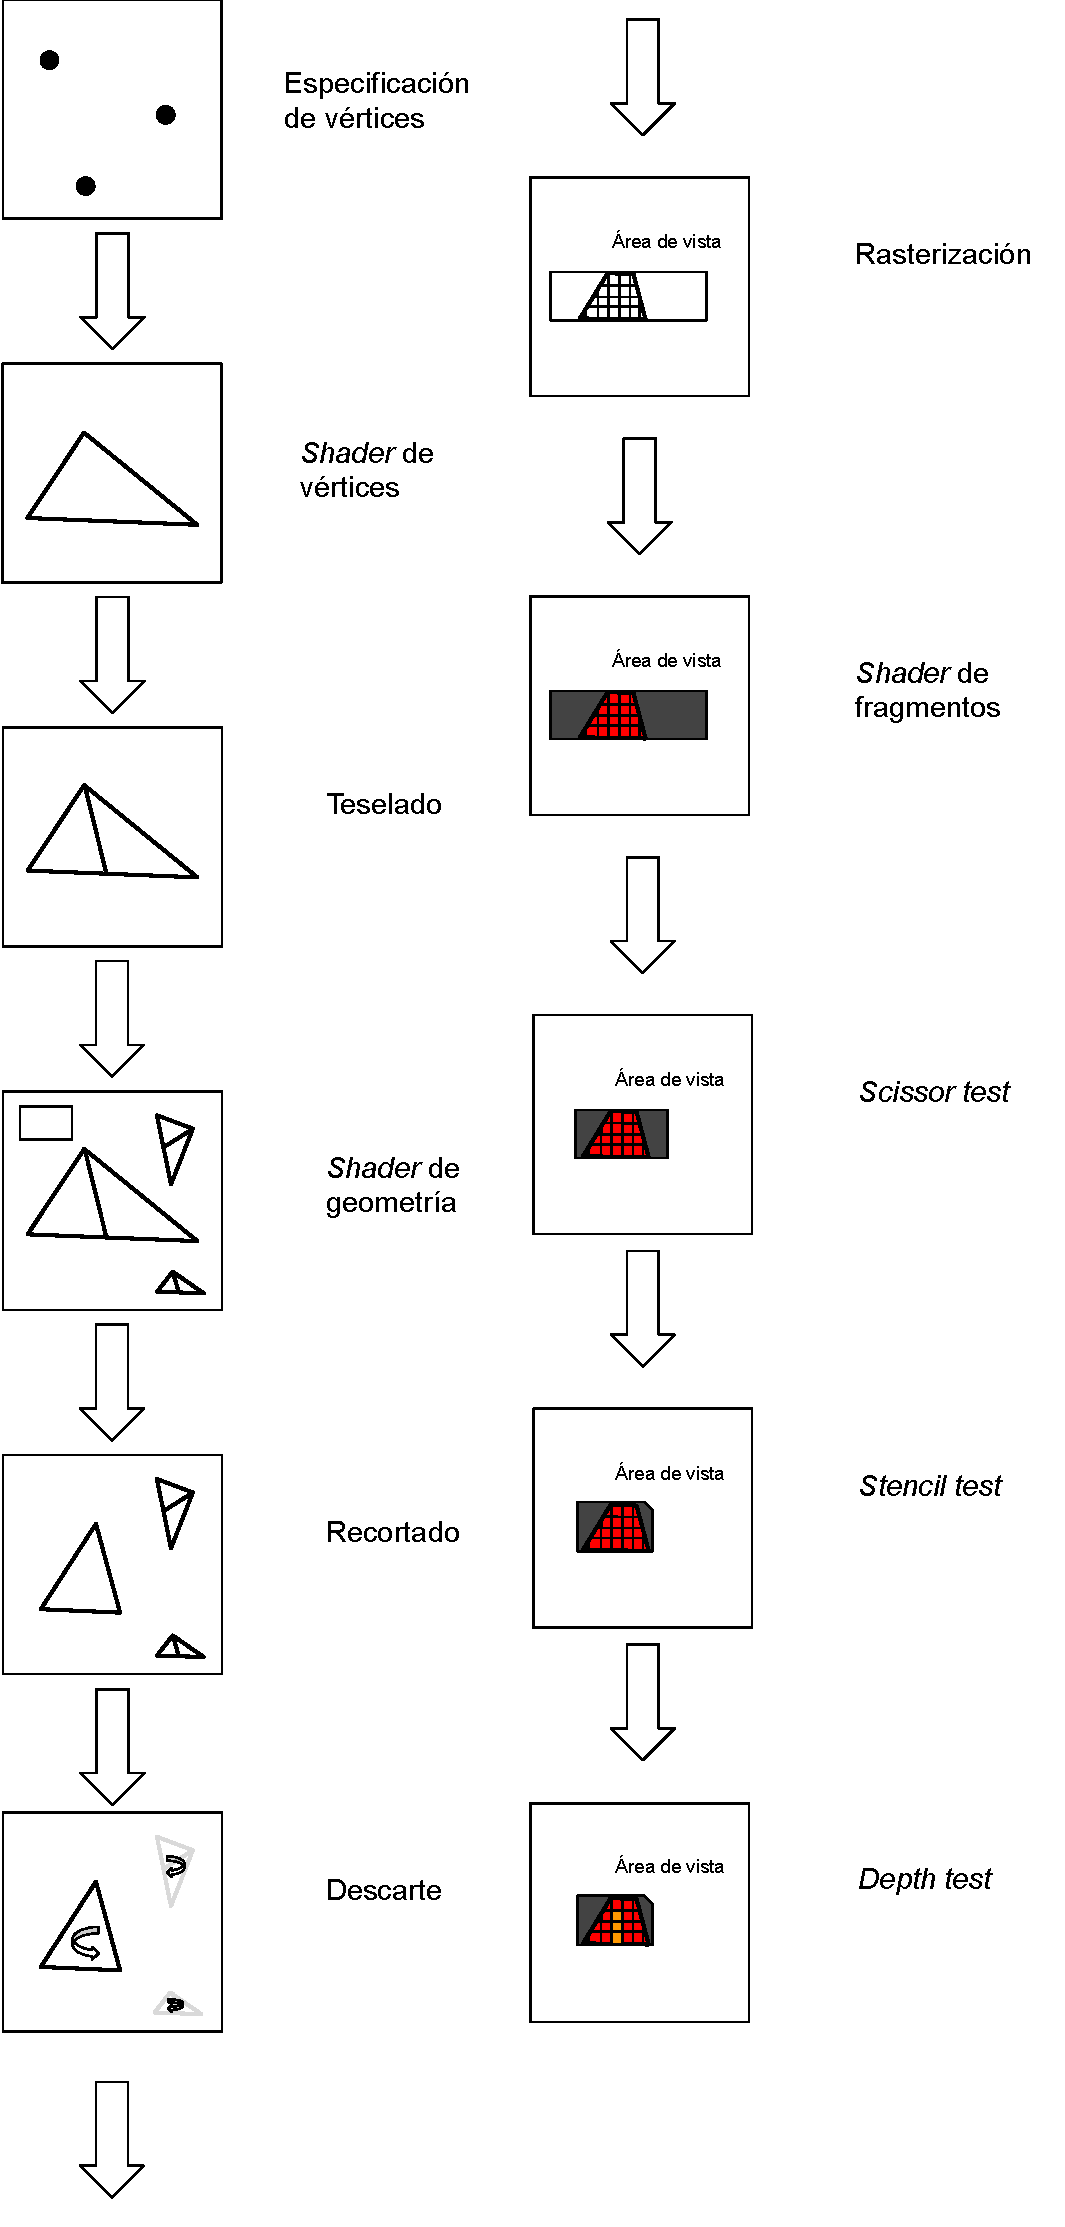
\includegraphics[width=0.55\linewidth]{assets/OpenGL}
	\captionof{figure}{El \textit{rendering pipeline} de OpenGL}
	\label{img:pipelinegl}
\end{figure}

Esta técnica de dibujado es extremadamente rápida, además, la mayoría de dispositivos contienen hardware especializado capaz de acelerar estos cálculos, comúnmente conocidos como Unidades de Procesamiento Gráfico (o GPU por sus siglas en inglés). Con el objetivo de aprovechar este hardware [Cohen y Greenberg \cite{Cohen}] idearon el método del hemi-cubo para el cálculo de factores de forma.

\subsubsection{El método del hemi-cubo}

El hardware optimizado para realizar operaciones de rasterización tiene la capacidad de proyectar escenas tridimensionales en imágenes planas a gran velocidad. 

El método original de cálculo de factores de forma propone la proyección de la escena una hemiesfera centrada en $S_{i}$, sin embargo los modelos de proyección utilizados no lo permiten. Por esto es necesario proyectar la escena a un hemi-cubo centrado en $S_{i}$, esto supone el dibujado de cinco superficies planar, y por tanto puede ser realizada utilizando la rasterización.

Para utilizar el hardware eficientemente consideraremos que se calcula una fila completa de $\mathbf{F}$, esto implica que dado el parche $S_{i}$, se calcula simultáneamente los factores de forma desde $S_{i}$ al resto de las superficies restantes. 

Este método aprovecha el buffer de profundidad (Z-buffer), para la correcta determinación de visibilidad entre parches tomando en cuenta los fragmentos proyectados para los elementos que se encuentren más cercanos al parche $S_{i}$.

Este algoritmo, propuesto originalmente por [Cohen y Greenberg] en \citeyear{Cohen}, propone rasterizar la escena tridimensional en cinco texturas correspondientes a las caras de un hemi-cubo. Para cada fragmento renderizado se sumará un valor diferencial del factor de forma, que dependerá de la posición del píxel en el hemi-cubo en relación a el hemiesferio que este aproxima.  Esta suma genera una fila de la matriz $\mathbf{F}$, específicamente la fila $\mathbf{F}_{i}$, como se puede observar en la Figura \ref{img:ff}.

Por tanto, podremos definir:

\begin{equation}
	\mathbf{F}_{ij} = \sum_{q=1}^{R} \delta{F_{q}}
	\label{eq:ffgreenberg}
\end{equation}
donde:
\begin{itemize}
	\item $R$ es la cantidad de píxeles correspondientes a la superficie $S_{j}$ que cubren el hemi-cubo.
	\item $\delta{F_{q}}$ el diferencial de factor de forma asociado al píxel del hemi-cubo $q$.
\end{itemize}

\vspace{5mm}
\begin{figure}[!ht]
	\centering
	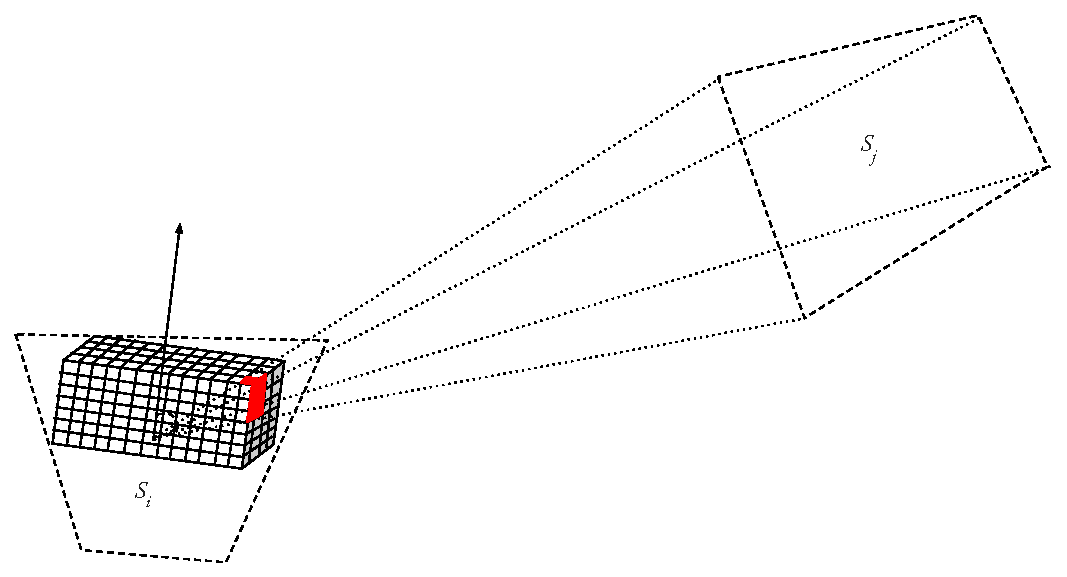
\includegraphics[width=0.8\linewidth]{assets/Hemicube}
	\captionof{figure}{Representación gráfica del método del hemicubo}
	\label{img:ff3}
\end{figure}

Los diferenciales de factores de forma deben corregir la deformación introducida con el cambio de proyección desde una hemiesfera a un hemi-cubo. Para ello, para cada píxel que compone el hemi-cubo es necesario calcular la proporición de área que este término ocupa en el hemiesferio unitaria.

Para la cara superior, los diferenciales se calculan como (ver referencias en la Figura \ref{img:deltaff}):

\begin{equation}
	\delta{F_{q}} = \frac{\cos{\phi_{i}}\cos{\phi_{j}}}{\pi{r^{2}}} \delta{A} = \frac{\delta{A}}{\pi({x^{2} + y^{2} + 1})} 
\end{equation}

Para las caras laterales, la fórmula dada es:

\begin{equation}
\delta{F_{q}} = \frac{\cos{\phi_{i}}\cos{\phi_{j}}}{\pi{r^{2}}}\delta{A} = \frac{z\delta{A}}{\pi({x^{2} + z^{2} + 1})}
\end{equation}

\begin{figure}[H]
	\centering
	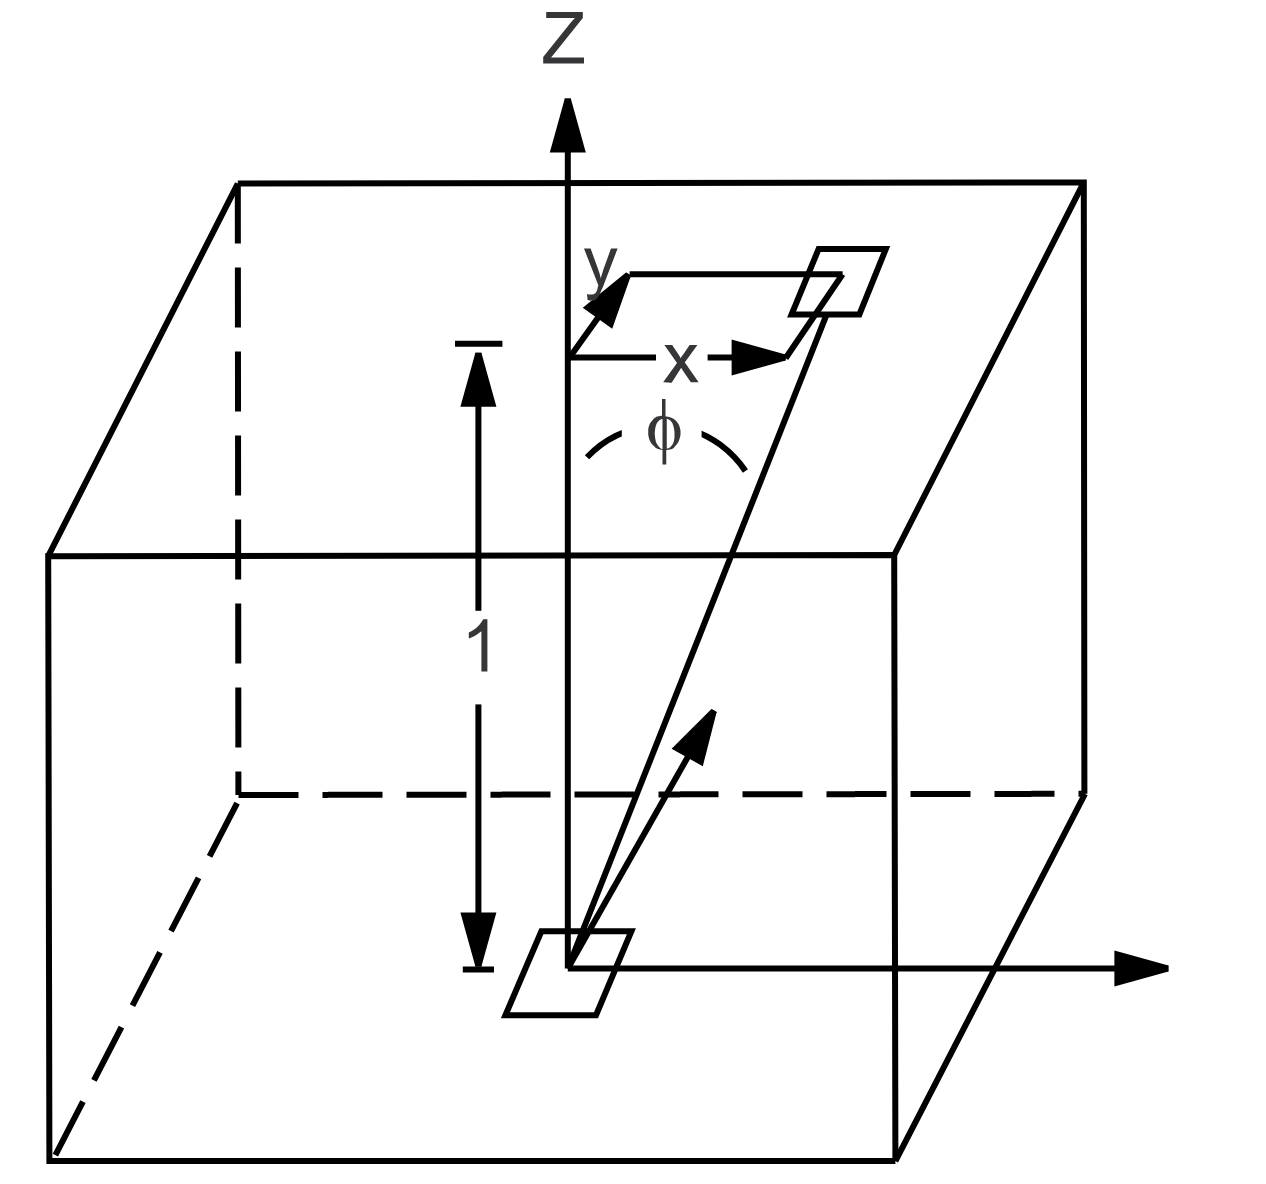
\includegraphics[width=0.4\linewidth]{assets/deltaff}
	\captionof{figure}{Representación gráfica de los ejes considerados para el factor de corrección de los factores de forma}
	\label{img:deltaff}
\end{figure}


\subsection{Trazado de rayos}
\label{sec:raytracing}

Otra de las técnicas de simulación de iluminación existente es el ray tracing que consiste en el cálculo de la intersección de una semi-recta (a la que denominaremos rayo) con la geometría de la escena, (cada uno de estos rayos simulará un haz de luz.

Para cada uno de los rayos emitidos, se determinará el punto de intersección más cercano. Dada la primitiva geométrica interceptada, es posible integrar el resultado intermedio al resultado final, dependiendo del modelo de iluminación utilizado.

El trazado de rayos es una técnica efectiva [Kajiya \cite{Kajiya}] para resolver la ecuación del rendering, utilizando la técnica de \textit{trazado de camino} donde el haz de luz absorbe las propiedades de los materiales con los que interacciona. En este algoritmo, la integral se resielve con un método de Monte Carlo, donde cada rayo representa una muestra estadísticamente independiente.

\subsubsection{El método del hemiesferio}

El algoritmo de ray tracing puede ser utilizado par ael cálculo de factores de forma, en particular para resolver la doble integral presentada en la Eq. \eqref{eq:ff}.

Es posible re-imaginar el problema original colocando una hemi-esfera unitaria en el centro de $S_{i}$ orientada en la direccción de la normal de la superficie.

El algoritmo propuesto por \citeauthor{Malley}  consiste realizar un muestreo de la cantidad de  rayos que parten desde el centro de $S_{i}$ e intersecan $S_{j}$. Las direcciones de los rayos serán determinadas a partir de la \textit{distribución del coseno} cuya función de densidad es $f(x) = \frac{1}{2}[1 + \cos((x-1)\pi)]$.

\begin{equation}
	\mathbf{F}_{ij} = \sum_{k=1}^{nMuestras} \frac{\beta(ray(S_{i},d), S_{j})}{nMuestras} 
	\label{eq:ffhemiesfera}
\end{equation}

donde:
	
	\begin{itemize}
		\item  $d$ sigue la distribución coseno.
		\item $\beta(r, S_{x})$ toma el valor 1 si el rayo $ray(S_{i},d)$ interseca a $S_{j}$ o $0$ en otro caso.
	\end{itemize}

\vspace{5mm}
\begin{figure}[H]
	\centering
	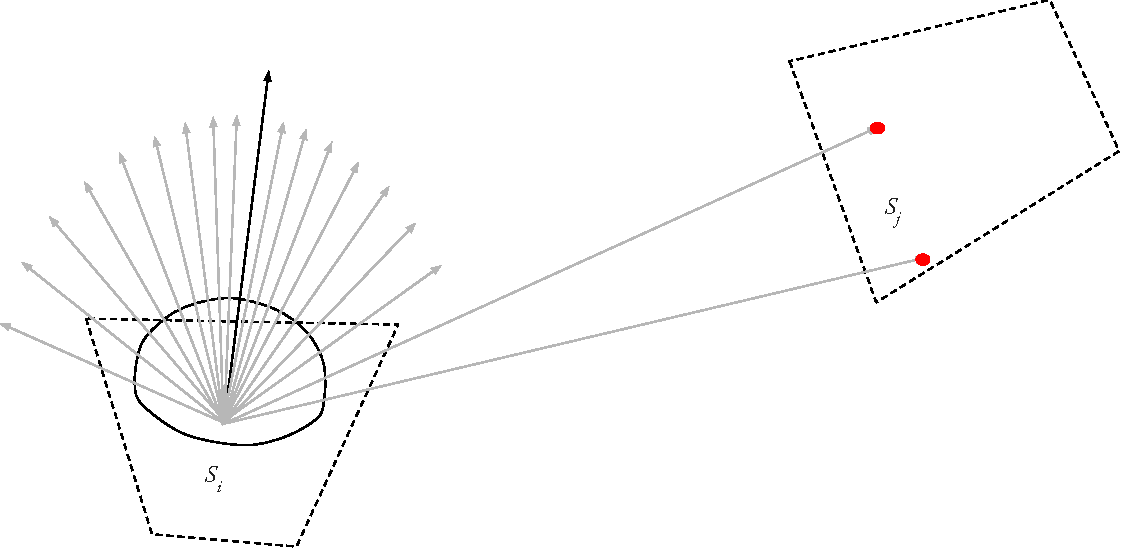
\includegraphics[width=\linewidth]{assets/Raytracing}
	\captionof{figure}{Representación gráfica del método de método de trazado de rayos para el cálculo de factores de forma}
	\label{img:ff}
\end{figure}

Cabe destacar que, no es necesario utilizar una distribución de probabilidad con valores aleatorios o pseudo-aleatorios, sino que, si la cantidad de rayos utilizados es la suficiente y además se utiliza una función que distribuya correctamente cada rayo, los resultados obtenidos se aproximan a los reales.

Para esto, pueden utilizare otras distribuciones para la dirección de traza. Particularmente, una de ellas es la propuesta por [\citeauthor{Beckers} \cite{Beckers}], presenta un método general de teselación de discos y hemi-esferas. Es desacable el hecho de que la propuesta para hemiesferas genera un conjunto de celdas de igual área que comparten la misma relación de aspecto. Esto hace que el método presente una calidad adecuada para la elección de las direcciones en la que se trazaran los rayos.

\section{Superficies especulares}

Originalmente, el método de cálculo de la radiosidad asume que todas las superficies son reflectores lambertianos, lo que supone que solo existirán reflexiones difusas cuando la luz interactúa con ellas. Sin embargo, en la mayor parte de las escenas del mndo real es necesario simular reflexiones especulares correctamente para obtener resultados que se asemejen a la realidad.

Por ello existe la extensión del método para superficies especulares o refractantes propuesto por [\citeauthor{Sillion} \cite{Sillion}]. Los autores proponen extender el significado del término \textit{factor de forma} a más que una mera relación geométrica entre parches. El nuevo factor de forma $\mathbf{F}_{ij}$ corresponde a la proporción de energía que deja la superficie $i$ y llega la superficie $j$ luego de un número de reflexiones y refracciones especulares.

Esto modifica completamente los algoritmos de cálculo de factores de forma. Los autores proponen un algoritmo de  que cálculo consiste en el trazado de rayos desde $S_{i}$ en una dirección arbitraria $d$ bien distribuida.  Luego, una vez que se conozca el camino trazado se distribuirá el valor final del factor de forma dependiendo en la cantidad de superficies con las que interaccione el rayo y sus coeficientes especulares como se observa en la Figura \ref{img:caminoespecular}.

\vspace{5mm}
\begin{figure}[H]
	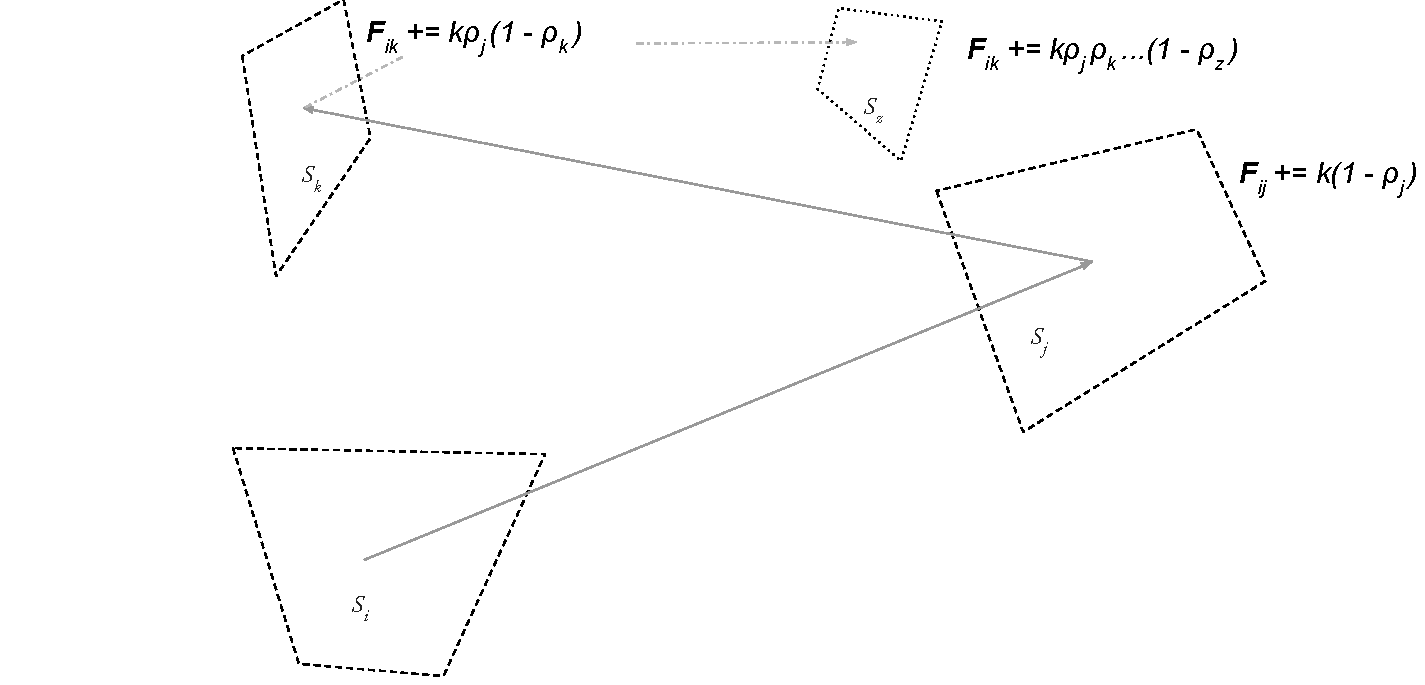
\includegraphics[width=1\linewidth]{assets/extended}
	\captionof{figure}{Representación gráfica del cálculo del factor de forma extendido donde $k = \frac{1}{N}$, con $N$ muestras tomadas.}
	\label{img:caminoespecular}
\end{figure}

\section{Cálculo del vector de radiosidades}
\label{sec:vrad}

Luego de computar la matriz $\mathbf{F}$ y dado los vectores de emisiones $E$ y reflexiones $\rho$, resta computar el vector de radiosidades correspondiente para cada parche, denominado $B$.

Recordando la Eq. \eqref{eq:radiosity}, es posible deducir el problema al sistema de ecuaciones dado por:

\begin{equation}
	E = (\mathbf{I} - \mathbf{RF})B
\end{equation}

Los estudios de álgebra lineal modernos permiten la resolución de sistemas de ecuaciones de forma optimizada, dependiendo de las propiedades observadas.

Recordando las propiedades en la Sección \ref{propsff}, podemos observar que:

\begin{itemize}
	\item $\sum_{j=1}^{N} \mathbf{F}_{ij} \leq 1 \forall{i \in [1,N]}$
	\item $\rho_{i} \leq 1 \rightarrow \sum_{j=1}^{N} \mathbf{R}_{ij} \leq 1 \forall{i \in [1,N]}$
\end{itemize}

Esto implica que las entradas de $\mathbf{RF}$ s\texttt{}on siempre menores a $1$, por tanto la matriz $(\mathbf{I} - \mathbf{RF}) = M$ es diagonal dominante ya que $\sum_{j=1}^{N}|R_{ij}F_{ij}| \le 1 \forall i \in [1, N]$ y $R_{ii}F_{ii} = 0  \forall  i \in [1,N]$. Esto garantiza la convergencia del uso de métodos de resolución iterativos o de factorización, como el algoritmo de Gauss-Seidel o la factorización LU.

Aunque los algoritmos clásicos de resolución de sistema de ecuaciones aplican a este problema, existen optimizaciones que hacen que su resolución se pueda aproximar de manera razonable con un costo computacional muy menor. Para ello, considerando que la matriz $\mathbf{F}$ es diagonal dominante, podemos utilizar la equación \ref{eq:iterativo} pues el \textit{residuo} (el término agregado en cada iteración) se reduce de la siguiente forma: $\left\|\mathbf{RF}B^{(i+1)}\right\| < \left\|\mathbf{RF}B^{(i)}\right\|$. El método planteado en la Eq. \eqref{eq:iterativo} es el método de Jacobi.

\begin{equation}
	B^{(i+1)}  = \mathbf{RF}B^{(i)}  + E \text{ con }  B^{(0)} = E
	\label{eq:iterativo}
\end{equation}

Cabe aclarar, que el método planteado hasta el momento resuelve la radiosidad en un único canal. Es decir, no se toma en cuenta todo el espectro electromagnético de la luz, es por ello que puede establecerse una extensión del método. Esta extensión implica la existencia de tres vectores de reflexión, uno para cada canal \textit{RGB} (del inglés \textit{Red - Green - Blue}). Por tanto es necesario que se resuelvan tres y no un único sistema de ecuaciones, aunque es posible destacar que la matriz $\mathbf{F}$ permanece constante pues depende de la geometría de la escena. El único cambio en el sistema surge en la matriz $\mathbf{R}$ que pasará a depender del canal seleccionado: $\mathbf{R}_{c}$.

\section{OpenGL}

Con el objetivo de proveer interfaces estandarizadas para el uso de tarjetas gráficas y los distintos algoritmos relacioandos a la rasterización existen un conjunto de interfaces que abstraen los recursos necesarios (hardware, sistema operativo). En el contexto de este proyecto, se estudia el uso de Open Graphics Library (OpenGL).

OpenGL es una especificación de una Interfaz de Programación de Aplicación (API por sus siglas en inglés) diseñada por la organizción Khronos Group. Su cometido es el dibujado de gráficos bidimensionales o tridimensionales utilizando el método de rasterización (ver Sección \ref{sec:rasterizacion}). Los distintos fabricantes de Sistemas Operativos y tarjetas gráficas proporcionan implementaciones que se ajusten al hardware específico. Esta abstracción facilita la compatibilidad de las aplicaciones independientemente del hardware donde sean ejecutadas.

\subsection{Arquitectura}
La arquitectura base de la bibliotecta es de cliente/servidor (ver Figura \ref{img:gpucpugl}). El cliente es la aplicación que invoca funciones para el dibujado de gráficos y es ejecutado en la CPU. El servidor, que es ejecutado en la GPU, almacena los distintos buffers y ejecuta las funciones necesarias.

El cliente modifica los atributos a través de invocaciones a las funciones de prefijo \verb|gl|, identificando el recurso afectado con valores enumerados (por ejemplo, \verb|GL_TEXTURE_2D| representa un conjunto de imágenes bidimencionales). Dado que la biblioteca es implementada como una máquina de estado, los atributos son recordados hasta que sean modificados nuevamente.

Estas invocaciones no son ejecutadas inmediatamente, sino que de forma similar a un buffer de entrada/salida son almacenados para ser ejecutados cuando sea necesario, es decir, cuando se requiera el dibujo de una nueva imagen. Esto hace que la ejecución de comandos sea asíncrona, y por tanto mejora el rendimiento previniendo la sincronización entre la CPU y GPU.

\vspace{5mm}
\begin{figure}[h]
	\centering
	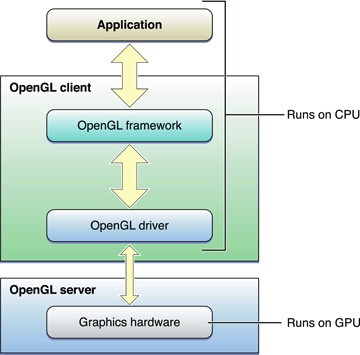
\includegraphics[width=.4\linewidth]{assets/cpu_gpu}
	\caption{Vista general de la arquitectura de OpenGL}
	\label{img:gpucpugl}
 \end{figure}

\subsection{Extensiones}
La inicialización de la máquina de estados depende directamente de la creación de un contexto que será utilizado para almacenar los datos. Este proceso depende fuertemente de la plataforma donde se ejecute la aplicación, que depende entre otros del sistema operativo y/o el hardware utilizado. Por este motivo, existen bibliotecas que manejan la creación del contexto en diversas plataformas como SDL y GLFW.
	
\section{Embree}

Los distintos algoritmos para evaluar la intersección entre superficies y rayos han evolucionado a gran velocidad, introduciéndose los conceptos de volumen envolvente y jerarquías de escena. Esto resulta en un gran re-trabajo al momento de implementar algoritmos que se basan en el trazado de rayos de forma eficiente. Es por ello, que de manera similar a las APIs de dibujado de gráficos acelerados por hardware existen interfaces que facilitan la aceleración del trazado de rayos. En particular, Embree es una biblioteca creada por Intel con este propósito.

La biblioteca expone un conjunto de funciones para realizar el trazado de rayos acelerado a través de componentes de hardware y software mediante la utilización del conjunto de instrucciones del paradigma SIMD (del inglés Single Instruction - Multiple Data), donde una única instrucción es ejecutada sobre un gran conjunto de datos (por ejemplo, la ejecución concurrente de un conjunto de multiplicaciones en punto flotante a nivel de CPU) y la generación de estructuras de aceleración, como las BVH (del inglés \textit{Bounding Volume Hierarchies}). La arquitectura de la aplicación, diagramada en la Figura \ref{img:embree}, demuestra los distintos algoritmos propuestos para la generación de estructuras de aceleración y algoritmos de intersección eficientes.

La biblioteca resuelve un conjunto de dificultades normalmente encontradas en todas las aplicaciones de algoritmos que involucren el trazado de rayos, entre ellas:

\begin{itemize}
	\item \textbf{Multi-hilo:} Con el objetivo de ejecutar distintos kernels de traza de rayos de forma concurrente, la biblioteca provee de funciones \textit{thread-safe} para el dibujado y la generación de estructuras de aceleración.
	\item \textbf{Vectorización:} Con el objetivo de optimizar el uso de la CPU, la biblioteca vectoriza los cálculos necesarios para aprovechar las instrucciones SIMD.
	\item \textbf{Soporte para múltiples CPUs:} La biblioteca provee de una capa de abstracción independiente del hardware donde se utilice.
	\item \textbf{Conocimiento del dominio extenso:} Dado que la biblioteca implementa las estructuras de aceleración y los algoritmos de intersección no es necesario tener un conocimiento completo del dominio para construir aplicaciones utilizando trazado de rayos.
	\item \textbf{Manejo eficiente de la memoria:} Para la visualización de escenas con gran cantidad de primitivas.
\end{itemize}

\vspace{5mm}
\begin{figure}[H]
	\centering
	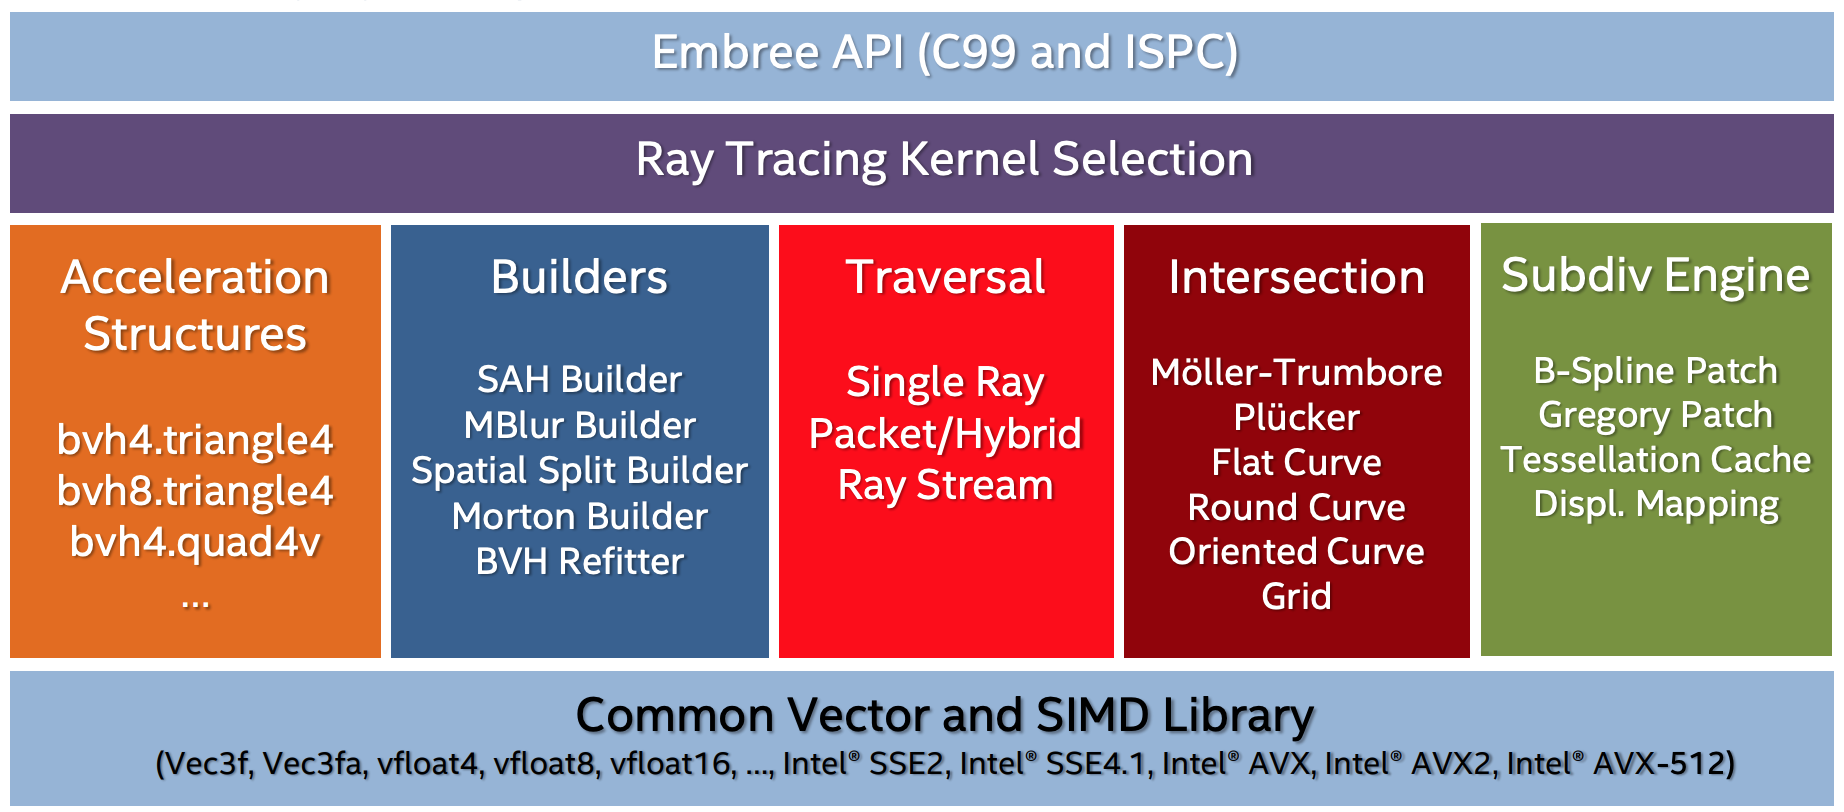
\includegraphics[width=.8\linewidth]{assets/embree}
	\caption{Vista general de la arquitectura de Embree}
	\label{img:embree}
\end{figure}

\section{Trabajos relacionados}

En esta sección se discuten alternativas propuestas para resolver el cálculo de la iluminación global en escenas con materiales difusos y especulares.

El algoritmo propuesto por [Shirley \cite{Shirley}] calcula la iluminación difusa utilizando dos pasadas. Este algoritmo difiere del propuesto por [Sillion y Pueach \cite{Sillion}] en el sentido que se consideran distintos modelos de fuentes luminosas con propiedades particulares (luces puntuales, direccionales, de área).

En la primer pasada, el algoritmo calcula la componente difusa de todos los rayos que rebotan en al menos una superficie especular. Este método calcula los caminos que seguirán los rayos de luz provenientes de fuentes luminosas, es decir, se discretiza la cantidad de rayos emitidos por una fuente luminosa, cada rayo representa una fracción de la energía emitida.

Cuando existe una intersección, se divide la energía entre los cuatro nodos más cercanos (estos nodos almacenan la radiosidad) a través de una estimación para calcular qué área ocupa cada uno de ellos, de esta manera es posible generar un mapa de radiosidad para la superficie. Dado que la iluminación directa (es decir, aquellos rayos que no se intersecan con superficies especulares) es calculada en la etapa de vista, solo es necesario computar los rebotes especulares, para ello se traza un número bajo de rayos distribuidos de forma uniforme para encontrar las zonas donde existan superficies especulares, luego se trazan rayos en esa dirección de forma "densa", que implica trazar una cantidad de rayos considerable en una dirección que no varía demasiado.

El segundo paso utiliza el método de radiosidad para calcular la iluminación difusa que involucra al menos dos superficies, nuevamente se omite la iluminación directa pues se calculará en la etapa de vista. Para ello, se emiten rayos desde cada supeficie utilizando la distribución del coseno de manera equivalente a la propuesta por \citeauthor{Malley}. 

Finalmente, cuando se dibuja la imagen final también se calcula la iluminación directa de forma estándar (ver [Whitted \cite{Whitted}]) sustituyendo el término de ambiente por el calculado en las pasadas anteriores.

Otro acercamiento al problema es el método propuesto de [Kok \cite{Kok}] es una extensión para parches que están formados por superficies de Bézier, estas son superficies delimitadas por curvas de nombre homónimo que para una superficie definida con $m$ puntos siguen la ecuación $c(u,v) = \sum_{i=0}^{m} c_{i}(v)B_{i}^{m}(u)$ donde $c$ es el vector de desplazamientos, y $B$ una función que genera la curva.

Los autores proponen la discretización de las superficies en puntos de muestreo dependiendo del área, luego simplemente se calcula el factor de forma de la superficie utilizando el método de la hemi-esfera, agregando los resultados para cada punto. En caso de que un rayo interseque una superficie especular, los autores proponen un método similar al de [Sillion y Puech \cite{Sillion}] donde se seguirá el camino del rayo mientras rebote en superficies especulares y arribe en una difusa, distribuyendo el factor de forma entre las superficies involucradas dependiendo del coeficiente de reflexión especular.

Una formulación distinta del problema, que también se focaliza en el uso de radiosidad es [Holly y Torrance \cite{Holly}]. Los autores proponen, nuevamente, un método de dos pasadas donde el factor de forma está compuesto por tres partes el factor de forma delantero y trasero. El primero, está intrínsecamente relacionado a la reflexión difusa y tiene el mismo comportamiento que el factor de forma definido por [Cohen \cite{Cohen}] mientras que el segundo se relaciona con el fenómeno de la refracción y es calculado integrando en el hemiesferio opuesta por la normal del parche. La última componente son los factores de forma de ventana, que contienen la información referente a la reflexión especular.

El método propone el uso del hemicubo para calcular los factores de forma delanteros, mientras que los traseros son calculados invirtiendo el hemicubo. Para calcular las componentes especulares, se utiliza un método similar al propuesto en el dibujado de portales, con la salvedad de que se opta por duplicar la geometría simétricamente en lugar de simplemente trasladar la cámara.
  \chapter{Solución propuesta}
\label{ch:chap03}

\section{Alcance y objetivos}
\label{sec:alcance}

Este proyecto se centra en la implementación completa de una aplicación capaz de calcular tanto la matriz de factores de forma como el vector de radiosidad final. Comparando el rendimiento de los distintos métodos en \ref{ch:chap02}, en escenas compuestas por triángulos y cuadriláteros.

Los métodos involucrados incluyen:

\begin{enumerate}
 	\item Cálculo de factores de forma utilizando el hemi-cubo
 	\item  Cálculo de factores de forma utilizando trazado de rayos
 	\item Cálculo de factores de forma extendidos utilizando dibujado de portales
 	\item Cálculo de factores  de forma extendidos utilizando trazado de rayos
\end{enumerate}

Además, será necesario implementar una interfaz de usuario que facilite la carga, edición y visualización de los objetos que componen la escena y sus respectivas propiedades (geometría, emisión inicial, coeficientes de reflexión difusa y especular, y radiosidad). Se soportará la carga de datos geométricos y materiales utilizando el formato estándar \verb|Waveform|.

\section{Proceso de desarrollo}
\label{sec:procdes}

Dada la naturaleza del proyecto, fue deseable establecer una metodología de desarrollo para facilitar el proceso de seguimiento del progreso incluso cuando el equipo de desarrollo fue individual.

Para ello, internamente, se utilizó una metodología ágil de desarrollo similar a la conocida como \textit{Kanban}.

Los principios claves del método aplicado a este proyecto fueron:
\begin{itemize}
	\item La visualización sencilla del curso de trabajo (una lista de tareas a realizar conocida como \textit{Backlog})
	\item La limitación de las tareas en progreso.
	\item Dirigir y gestionar el flujo de trabajo implica la priorización de tareas a realizar dada una cantidad finita de recursos.
\end{itemize}

La gestión de las tareas a relizar se llevó a cabo en el respositiorio del proyecto, con tareas como las vistas en \ref{img:kanban}. Donde se consideran un conjunto de tareas:

\begin{itemize}
	\item Backlog: Las tareas a realizar, en orden de importancia.
	\item In progress: Las tareas actualmente en desarrollo.
	\item Done: Las tareas cuya funcionalidad fue completamente desarrollada y probada.
\end{itemize}

\vspace{5mm}
\begin{minipage}[h]{0.8\linewidth}
	\centering
	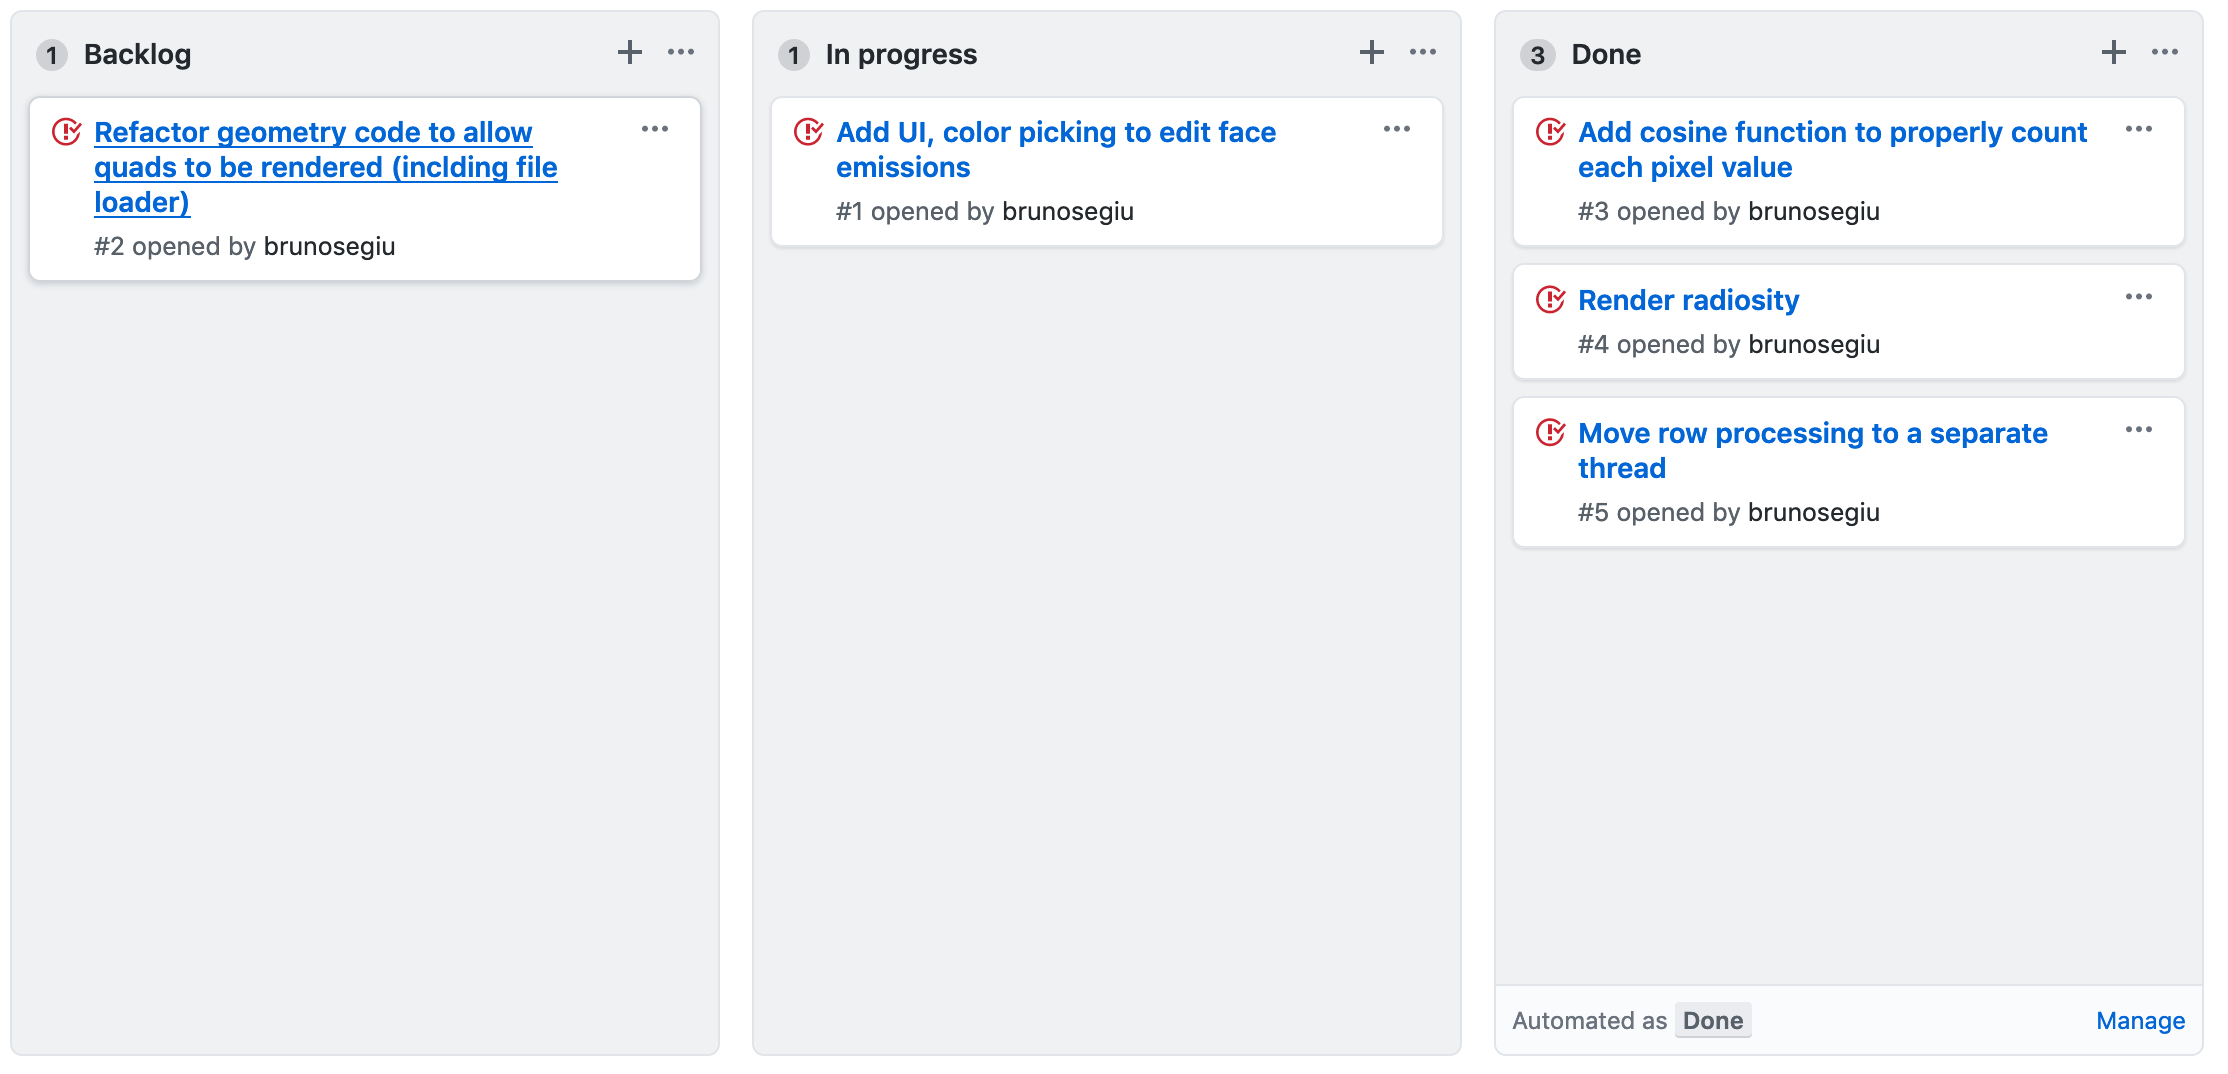
\includegraphics[width=\linewidth]{assets/kanban}
	\captionof{figure}{Tabla de Kanban utilizada en el proyecto}
	\label{img:kanban}
\end{minipage}

\section{Diseño}
\label{sec:disenio}

Con la finalidad de evitar el alto acoplamiento, facilitar la extensión y reducir la cantidad de errores de integración se tomó la decisión de utilizar distintos módulos y sub-módulos que ofrezcan un conjunto de funcionalidades bien definido utilizando programación orientada a objetos. Esta decisión permite el añadido de nuevas características y la optimización de ciertas funcionalidades independientemente de los demás módulos contruidos.

El diseño de la solución comprende dos componentes principales, la interfaz gráfica de usuario (GUI, en inglés) y el motor de renderizado.

\subsection{Motor de renderizado}
\label{sec:engine}

El paquete del motor de renderizado se compone de un conjunto de sub-módulos, el primero de ellos que maneja el pre-procesado de una escena, es decir, el cálculo de l matriz de factores de forma y la radiosidad. El siguiente conjunto de sub-módulos se ocupan del renderizado en tiempo real de la escena, así como la carga de modelos desde el disco duro, la modificación de materiales, entre otras funcionalidades detalladas en \ref{sec:ui}.

\subsubsection{Módulo de geometría}

El módulo de geometría encapsula la información de las escenas leídas desde el disco duro, además de adaptar y optimizar los formatos de las primitivas geométricas para ser utilizados en las APIs de dibujado de terceros. La clase \verb|Scene| \ref{img:geom} cargará distintos objetos desde el disco duro que serán manejados como una instancia de \verb|Mesh|.


\vspace{5mm}
\begin{minipage}[h]{0.7\linewidth}
	\centering
	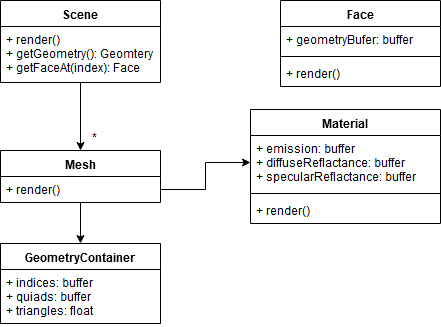
\includegraphics[width=\linewidth]{assets/geometry}
	\captionof{figure}{Módulo de manejo de geometría}
	\label{img:geom}
\end{minipage}

\subsubsection{Módulo de pre-procesado}

El módulo de preprocesado se compone de un controlador principal (\verb|PreprocessController| en la figura \ref{img:procesado}), que maneja el estado y la ejecución de  los comandos de los distintos \textit{pipelines} implementados que resuelven el cálculo de la radiosidad.

\vspace{5mm}
\begin{minipage}[h]{0.8\linewidth}
	\centering
	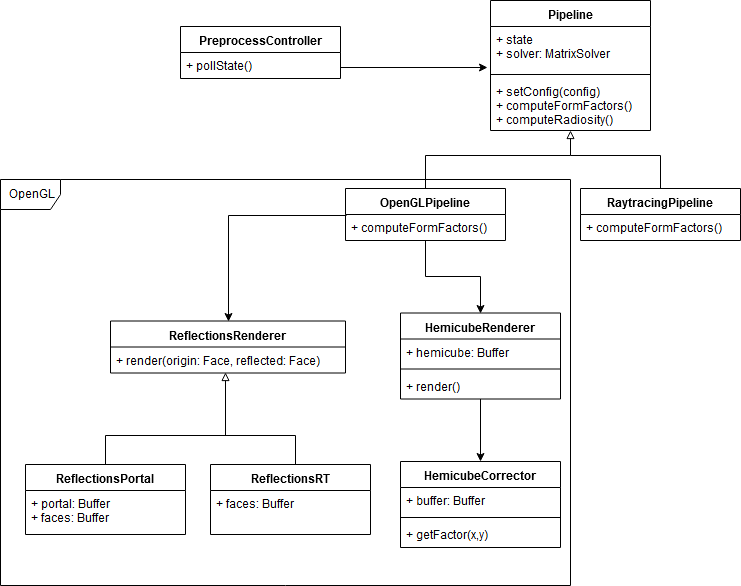
\includegraphics[width=\linewidth]{assets/preprocess}
	\captionof{figure}{Arquitectura del módulo de pre-procesado}
	\label{img:procesado}
\end{minipage}

Un pipeline es definido a partir de un conjunto de funciones ejecutadas en el siguiente orden:

\begin{enumerate}
	\item \verb|setConfig(scene, interpolator, reflections, n_channels, solver)|
	\item \verb|computeFormFactors()|
	\item \verb|computeRadiosity()|
\end{enumerate}

Donde \verb|computeFormFactors()| variará dependiendo del método de cálculo elegido (veáse \ref{img:procesado}), donde puede utilizarse el método del hemi-cubo o el de la hemi-esfera. El primero de ellos utilizará un \textit{pipeline} configurado utilizando una API de rasterización, mientras que el segundo utilizará una API capaz de calcular intersecciones utilizando \textit{trazado de rayos}.

La ejecución de \verb|computeRadiosity()| dependerá directamente de \verb|solver| seleccionará el algoritmo que calculará el vector de radiosidades para la escena.

\subsubsection{Módulo de visualización}

El módulo de visualización se encarga de renderizar la escena actual desde el punto de vista seleccionado por el usuario. Además, debe tener la capacidad de mostrar las distintas propiedades de los materiales como valor de emisión inicial, valor de reflexión especular, visualización de geometría para facilitar la edición de las propiedades de los objetos o sus caras. El proceso de dibujado comienza con el dibujante de la escena que dibujará un conjunto de imágenes correspondiente a las propiedades de los materiales \verb|SceneRenderer| en la figura \ref{img:vis}, luego un dibujante de texturas \verb|TextureRenderer| seleccionará y convertirá correctamente el resultado anterior a valores tres canales (RGB). El módulo de visualización siempre tendrá una textura bidimensional como parámetro de salida.

\vspace{5mm}
\begin{minipage}[h]{0.8\linewidth}
	\centering
	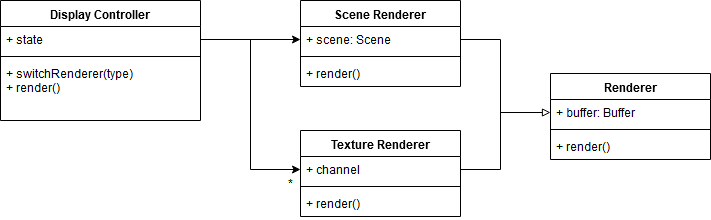
\includegraphics[width=\linewidth]{assets/display}
	\captionof{figure}{Arquitectura del módulo de visualización}
	\label{img:vis}
\end{minipage}

\subsection{Interfaz gráfica}

El módulo de visualización (UI) utiliza una arquitectura basada en el paradigma del \textit{bucle de eventos} \ref{img:ui}, consiste en un bucle que detecta y maneja los distintos eventos recibidos por el sistema. Este método es útil para el manejo sencillo de la concurrencia en sistemas con múltiples hilos en ejecución y es de fácil implementación pues procesa cada uno de los eventos completamente antes de procesar el siguiente

En alto nivel, el \textit{bucle de eventos} se compone de la siguiente forma:

 \begin{algorithmic}
 	\While{$queue.waitForEvent()$}
 		\State $queue.processEvent()$
 	\EndWhile
 \end{algorithmic}
 
 El  \textit{bucle de eventos} procesará todos los eventos de la aplicacación, lo que desencadena un conjunto de acciones que modificarán su \textbf{estado} de la interfaz de usuario. Este estado será dibujado por un conjunto de \textbf{componentes}, que no son más que presentadores del estado actual. Es decir, a partir de un conjunto de valores los presentarán en un formato gráfico adecuado y sencillo de comprender.

\vspace{5mm}
\begin{minipage}[h]{0.8\linewidth}
	\centering
	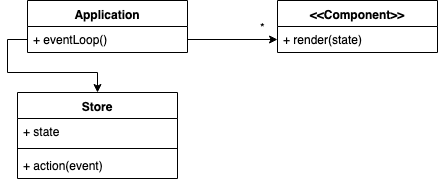
\includegraphics[width=\linewidth]{assets/ui}
	\captionof{figure}{Arquitectura general del módulo de interfaz de usuario}
	\label{img:ui}
\end{minipage}

\label{sec:ui}
  \chapter{Implementación}
\label{ch:chap04}

\section{OpenGL}
\label{sec:opengl-impl}

\subsection{Cálculo de factores de forma de la componente difusa}

El \textit{pipeline} de cáculo de factores de forma utilizando OpenGL se compone de tres etapas principales.

Etapa 1:

En primera instancia, se configurarán los \textit{buffers} de memoria necesarios para representar el hemi-cubo que se dibujará.

Para ello, se crea un \textit{Frame Buffer Object} en la GPU que estará compuesto de 5 texturas, cada una de ellas correspondiente a una de las caras a dibujar. Cabe destacar, que estas texturas se compondrán de dos imágenes, una de ellas contiene enteros sin signo que serán utilizados para representar un \verb|id| de cara parche de la escena y la restante contiene los valores de profundidad necesarios para el algoritmo del Z-Buffer.

Etapa 2:

En la segunda etapa se procede al renderizado y procesado de cada uno de los hemi-cubos. Para ello, se procede como en \ref{alg:hemicube}.

\begin{minipage}{\linewidth}
	\label{alg:hemicube}
	\begin{algorithmic}[H]
		\Function{$processHemicube$}{$face, hemicube$}
			\State $row \gets [0,...,0]$
			\Loop{$pixel \in hemicube:$}
				\State $factor \gets getHemicubeCorrection(pixel)$
				\State $seenFace \gets getFaceId(pixel)$
				\If{$isValid(seenFace)$}
					\State $row[seenFace] \gets + factor$
					\State $formFactorMatrix[face] \gets  row$;
			\EndLoop
		\EndFunction
		
		computeFormFactors() {
			bindHemicube()
			for (face in scene){
				alignCamera(face);
				clearBuffers();
				render(scene);
				hemicube = getHemicube();
				startThread(processHemicube, face, hemicube)
			}
		}
		
	\end{algorithmic}
\end{minipage}

El proceso de renderizado del hemicubo es realizado completamente en la GPU, sin embargo tiene características particulares que diferencial el proceso de otras implementaciones del algoritmo. 

Con el objetivo de tener el mejor rendimiento posible, se hace uso de los \textit{geometry shaders} para realizar una única llamada de dibujado por objeto. Además, como puede apreciarse en la figura \ref{img:statechangescost}, el método posibilita el cambio de \textit{render target} una única vez, al comienzo del dibujado como se ilustra en \ref{alg:hemicube} solo se realiza una única llamada de \textit{binding} del hemi-cubo .

\vspace{5mm}
\begin{minipage}[h]{\linewidth}
	\centering
	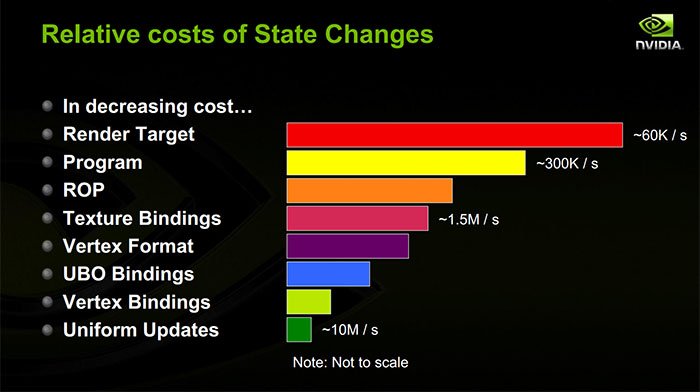
\includegraphics[width=\linewidth]{assets/statecosts}
	\captionof{figure}{Costo de cambios de estado en OpenGL. Fuente: Nvidia}
	\label{img:statechangescost}
\end{minipage}

El proceso consiste entonces en el dibujado de cinco texturas en simultáneo. 

\begin{enumerate}
	\item El \textit{vertex shader} es simplemente \textit{passthough} lo que signfica que conecta las entradas proveídas por la CPU con su salida.
	\item El \textit{geometry shader} genera cinco primitivas donde cada una estará en las coordenadas correspondientes a los frustums de las caras del hemicubo además de añadir un plano adicional de corte del dibujo necesario debido a la imposibilidad de que las caras laterales posean una resolución menor a la cara superior.
	\item El \textit{fragment shader} corregirá y escribirá el identificador de la cara detectada en la textura que le corresponda.
\end{enumerate}

\subsection{Cálculo de factores de forma de la componente especular}

\subsubsection{OpenGL}

\subsubsection{Embree}

\section{Embree}
\label{sec:embree-impl}

\subsection{Cálculo de factores de forma de la componente difusa}

\subsection{Cálculo de factores de forma de la componente especular}


\section {Interfaz de usuario}

  % !TeX spellcheck = es_ES
\chapter{Experimental}
\label{ch:chap05}

En este capítulo se muestran detalles de las pruebas realizadas, con el objetivo de determinar las características positivas y negativas de los algoritmos implementados en las dimensiones de rendimiento computacional y precisión de los resultados.

\section{Ambiente de prueba}
\label{sec:hardware}

A continuación, se presentan tanto el hardware utilizado en las pruebas (Tabla \ref{table:hardware}) así como las versiones del software utilizado (Tabla \ref{table:software}), de forma que los resultados puedan entenderse en términos relativos al entorno de ejecución utilizado.

\begin{table}[htbp!]
	\centering
	\begin{tabular}{l|l}
		Procesador & Intel i7 8700K - 12 CPUs - 3.7 GHz       \\
		\hline
		GPU        & Nvidia GeForce GTX 1070 Ti - 8 GiB  VRAM \\
		\hline
		RAM        & 32 GiB - 2667 MHz                        \\
		\hline
	\end{tabular}
	\caption{Características del hardware utilizado}
	\label{table:hardware}
\end{table}

\begin{table}[htbp!]
	\centering
	\begin{tabular}{l|l}
	SO & Windows 10 Pro        \\
		\hline
	Embree        & v3.5.2 \\
		\hline
		OpenGL        & v4.5  \\
		\hline
	\end{tabular}
	\caption{Características del entorno de desarrollo utilizado}
		\label{table:software}
\end{table}

\section{Escenas}
\label{sec:escenas}

Con el objetivo de obtener resultados comparables para los distintos algoritmos y configuraciones se plantea el uso de dos escenas particulares de prueba, con distintas variaciones en los materiales que componen cada una de ellas.


\begin{figure}[htbp]
	\centering
	\begin{subfigure}{0.45\textwidth}
		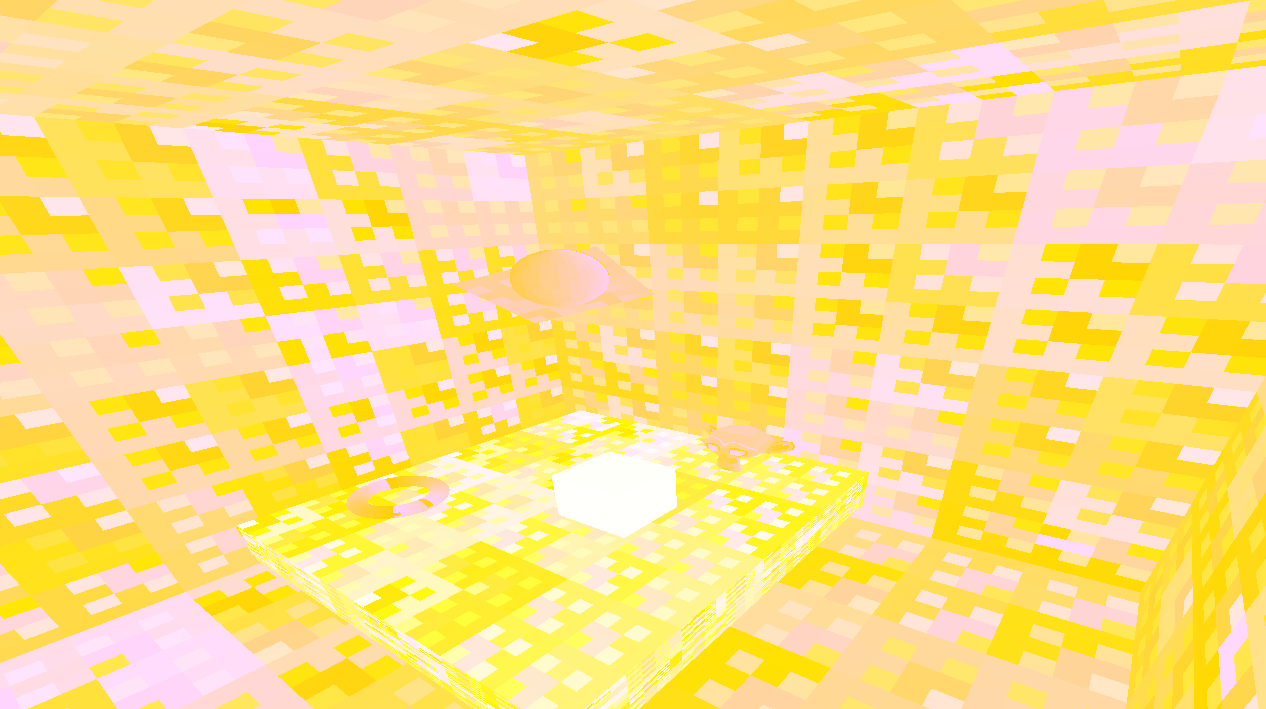
\includegraphics[width=1\linewidth]{assets/cornell}
		\caption{Lateral}
	\end{subfigure}
	\begin{subfigure}{0.45\textwidth}
		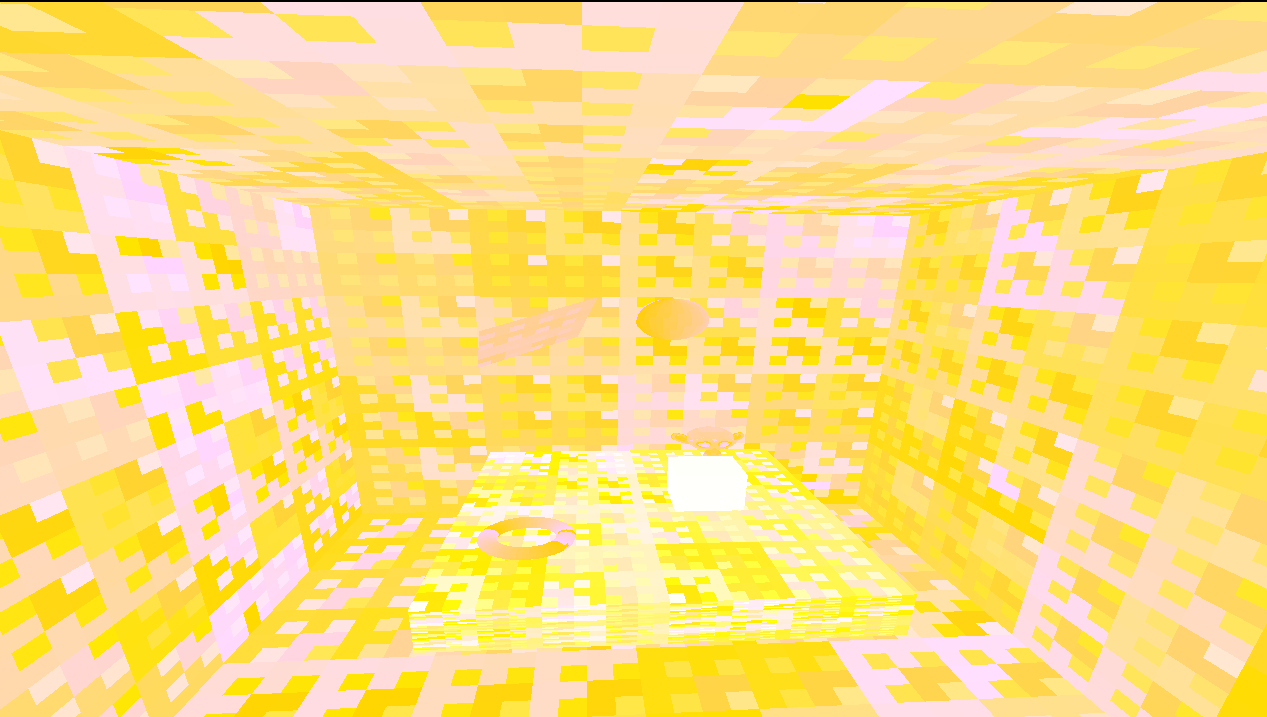
\includegraphics[width=1\linewidth]{assets/cornell2}
		\caption{Frontal}
	\end{subfigure}
	\caption{Vistas de la escena \textit{Conrnell Box}.}
	\label{img:cornell}
\end{figure}

Se denomina \textit{Escena - Cornell Box} a la mostrada en la Figura \ref{img:cornell}. Se basa en un tipo de escena comúnmente usado en el que se ubican objetos en el interior de un cubo, donde debajo están los objetos de prueba y en el nivel superior reside el objeto que emitirá luz. Esta escena cuenta con siete objetos: el cubo, una esfera que oficia de luz, y cinco objetos compuestos por diversas primitivas. En total, existen 12.922 polígonos de las cuales 96 son triángulos y 12.826 son cuadriláteros.

\begin{figure}[htbp]
	\centering
	\begin{subfigure}{0.45\textwidth}
		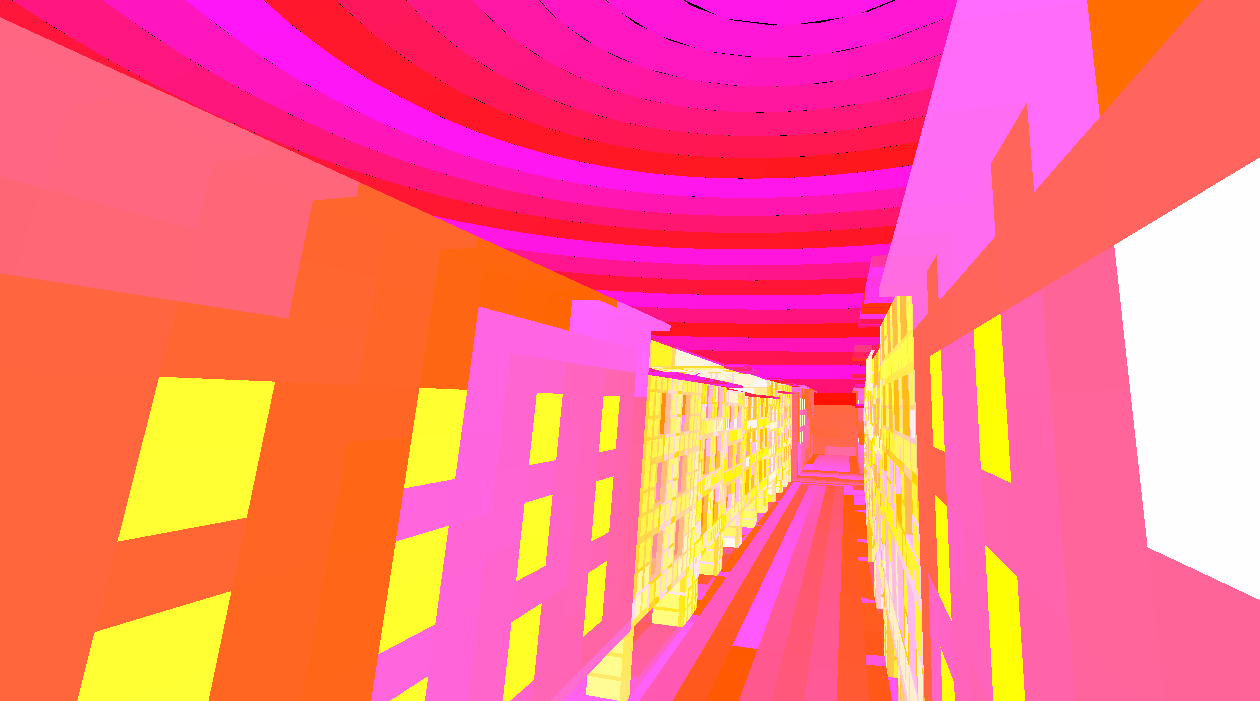
\includegraphics[width=1\linewidth]{assets/street1}
		\caption{Desde la ventana de una de las edificaciones}
	\end{subfigure}
	\begin{subfigure}{0.45\textwidth}
		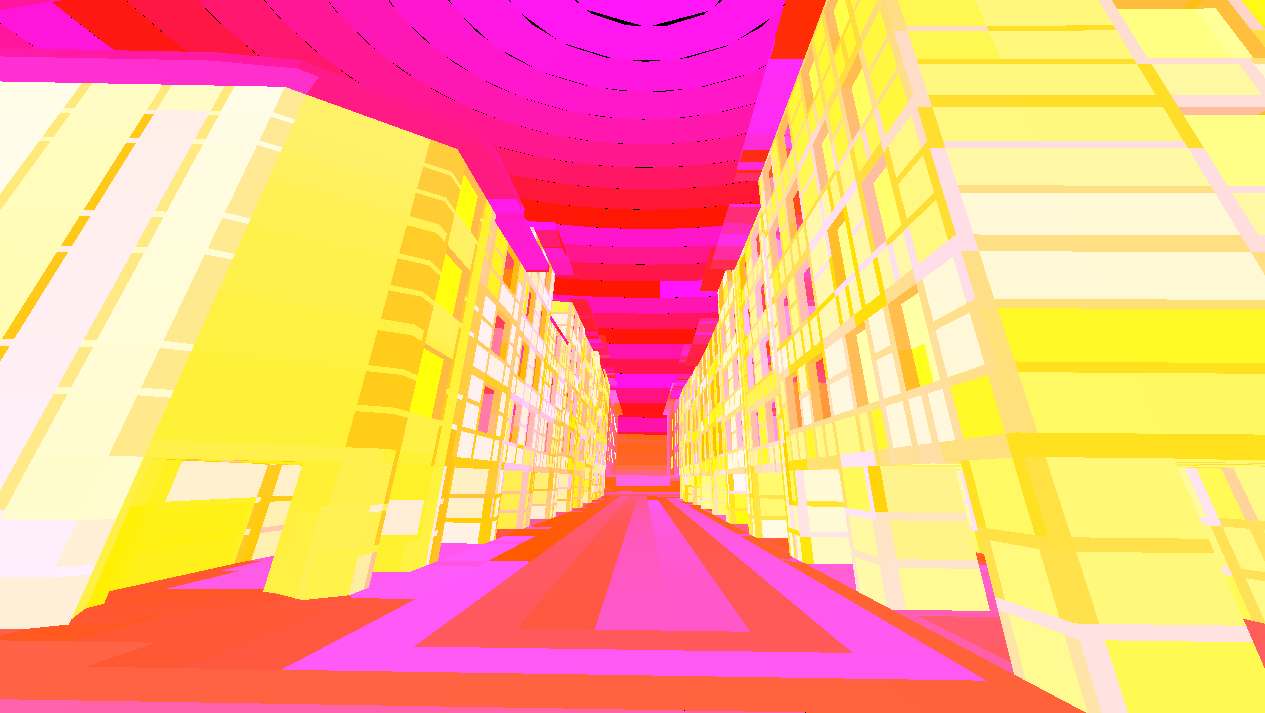
\includegraphics[width=1\linewidth]{assets/street2}
		\caption{Desde uno de los extremos de la calle}
	\end{subfigure}
	\begin{subfigure}{0.45\textwidth}
		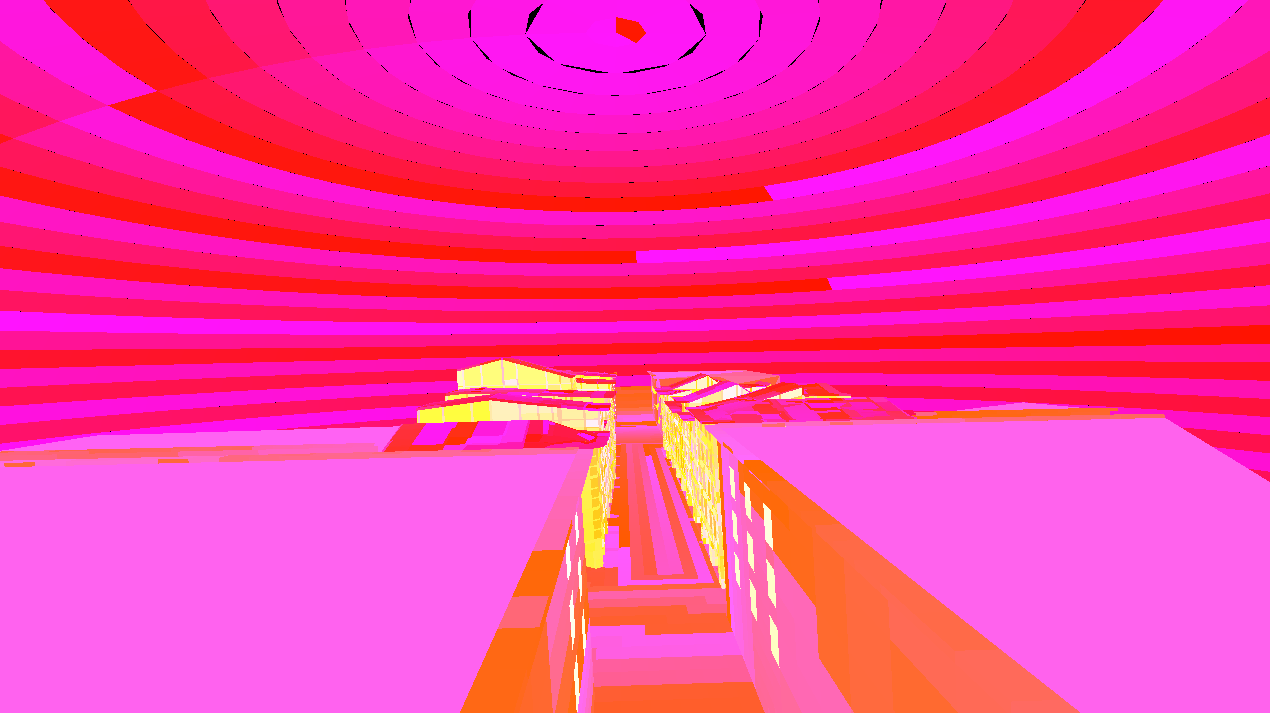
\includegraphics[width=1\linewidth]{assets/street3}
		\caption{Aérea I}
	\end{subfigure}
	\begin{subfigure}{0.45\textwidth}
		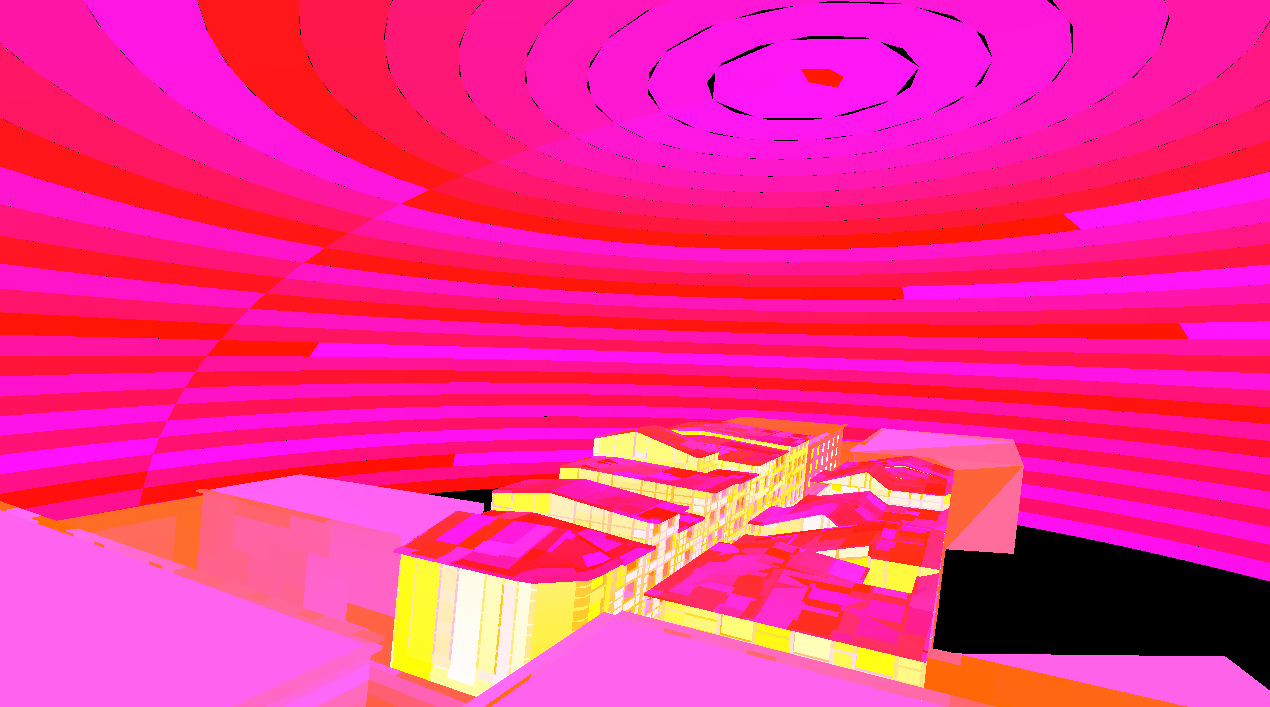
\includegraphics[width=1\linewidth]{assets/street4}
		\caption{Aérea II}
	\end{subfigure}
	\caption{Vistas de la escena \textit{Calle}.}
	\label{img:street}
\end{figure}

Se denomina \textit{Escena - Calle} a la referente a la Figura \ref{img:street}. La escena está constituida por dos objetos, el primero de ellos es una cúpula (hemisferio) subdividida en 2.407 cuadriláteros de igual área, cuyo objetivo es representar el cielo. Por otro lado, el segundo objeto es una representación de una porción de una calle en el barrio de Petit Bayonne, localizado en Bayona, Francia cuyas imágenes se aprecian en la figura \ref{img:streetcomp}. El modelo fue construido por Beniot, Acuña, et al. \cite{Benoit} con el objetivo de estudiar el fenómeno de la transferencia de calor a la escala de calle utilizando el método de elementos finitos. En total, la escena cuenta con 61.795 parches cuadrangulares.


\begin{figure}[htbp]
	\centering
	\begin{subfigure}{0.475\textwidth}
		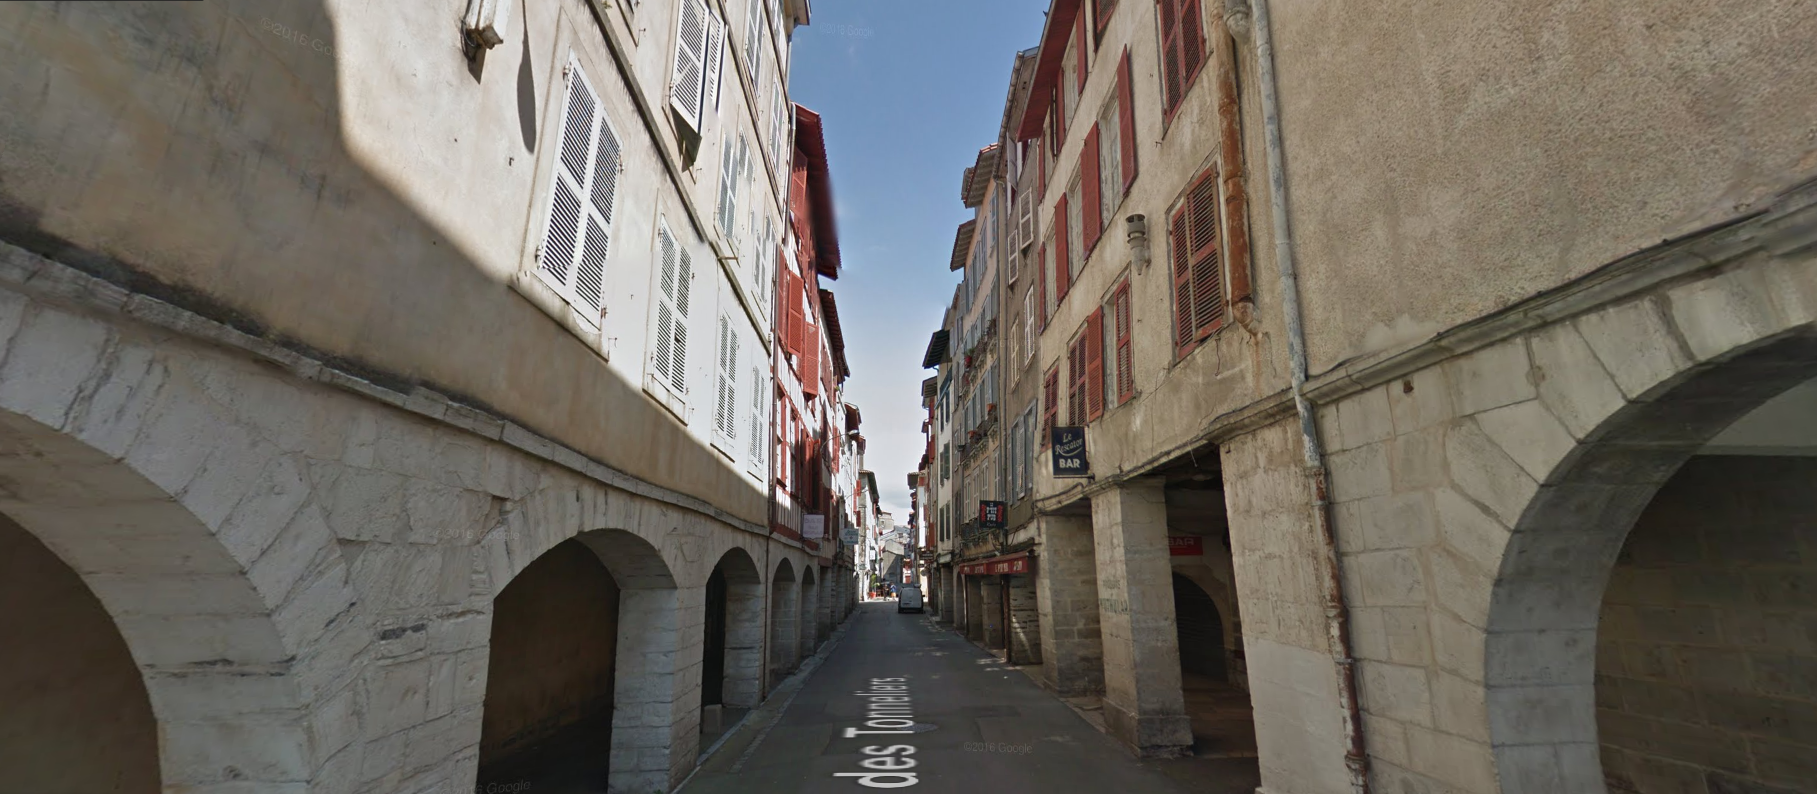
\includegraphics[width=1\linewidth]{assets/streetreal1}
		\caption{Sur - real}
	\end{subfigure}
	\begin{subfigure}{0.475\textwidth}
		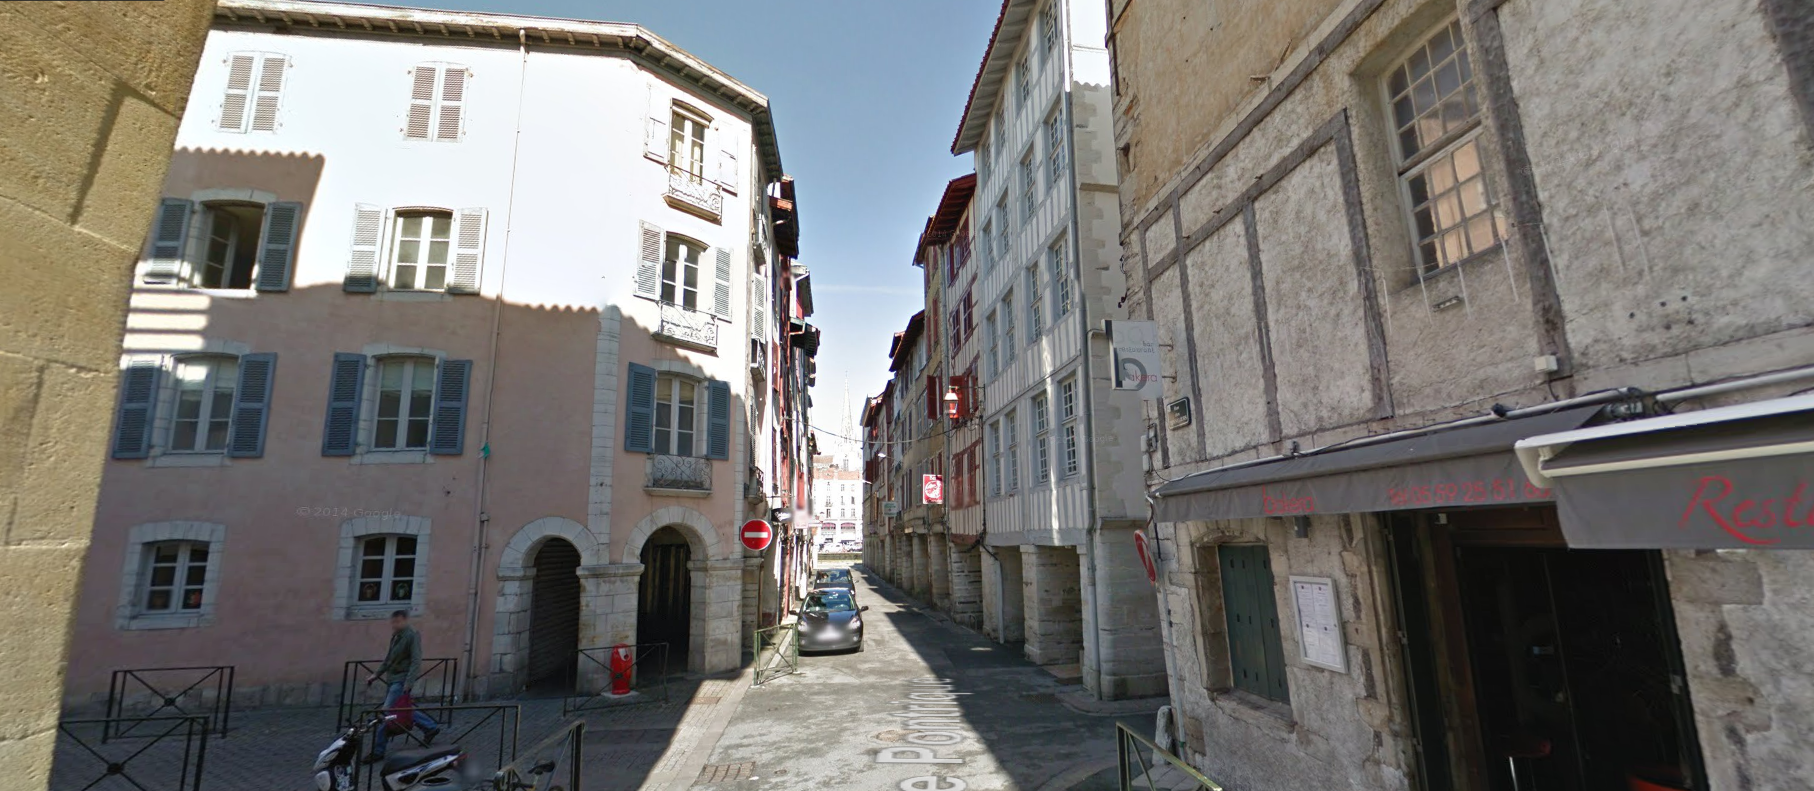
\includegraphics[width=1\linewidth]{assets/streetreal2}
		\caption{Norte - real}
	\end{subfigure}
	\begin{subfigure}{0.475\textwidth}
		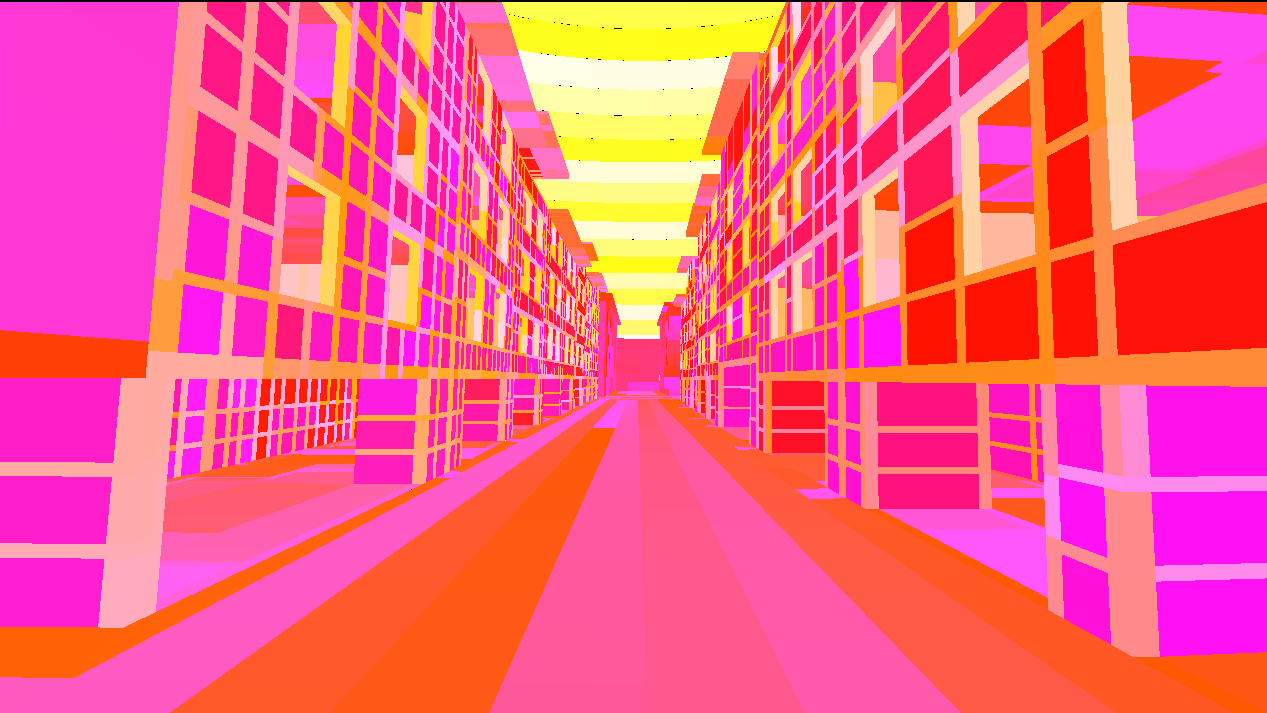
\includegraphics[width=1\linewidth]{assets/streetmodel1}
		\caption{Sur - modelada}
	\end{subfigure}
	\begin{subfigure}{0.475\textwidth}
		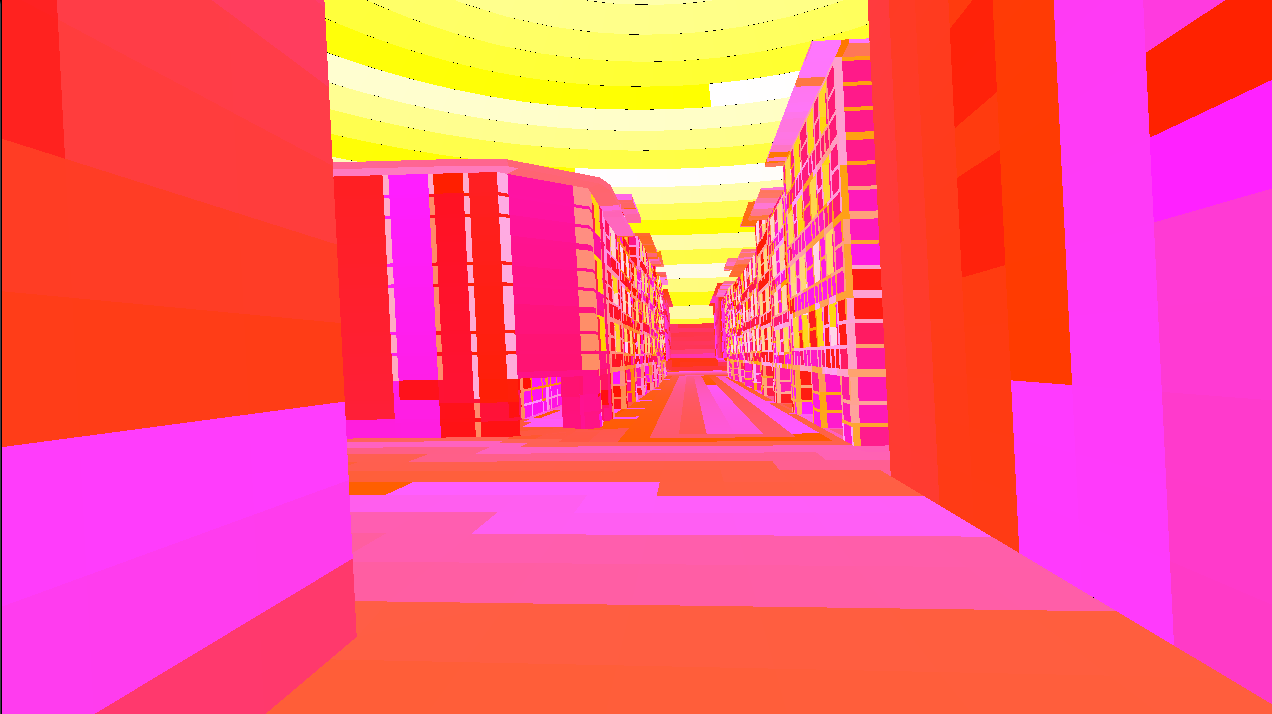
\includegraphics[width=1\linewidth]{assets/streetmodel2}
		\caption{Norte - modelada}
	\end{subfigure}
	\caption{Comparación entre el fotografías reales del modelo \textit{Calle} y su representación tridimensional.}
	\label{img:streetcomp}
\end{figure}

\section{Casos de prueba}
\label{sec:pruebas}

Se proponen casos de prueba utilizando las escenas descritas en la Sección \ref{sec:escenas}, compuestas por diversos materiales.

\subsection{Métricas consideradas}
\label{metricasestablecidas}
Con el objetivo de medir correctamente las ventajas y desventajas de cada método de cálculo de factores de forma simples y extendidos que se han propuesto, se define un conjunto de métricas para evaluar su optimalidad en distintas dimensiones. Cada dimensión se aplica dependiendo del caso considerado.

\begin{itemize}
	\item Rendimiento
		\begin{itemize}
			\item Tiempo de ejecución: Se registra el tiempo empleado en calcular completamente la matriz de factores de forma.
		\end{itemize}
	\item Matriz de factores de forma: Se compara la matriz de control $\mathbf{F_{C}}$, calculada utilizando la técnica de trazado de rayos con una gran resolución (3.145.728 rayos).
		\begin{itemize}
			\item Error relativo promedio por fila: $Ep_{i} = \sum_{j=1}^{N} \frac{|\mathbf{F_{C}}_{ij} -\mathbf{F}_{ij}|}{N \mathbf{F_{C}}_{ij}}$
			\item Error relativo máximo por fila: $Em_{i} = \max_{j=1}^{N}\frac{|\mathbf{F}_{ij} -\mathbf{Fc}_{ij}|}{\mathbf{F_{C}}_{ij}}$
		\end{itemize}
	\item Vector de radiosidad (dado el vector $B$, y el vector de control $Bc$, calculado a partir de la matriz de factores de forma $\mathbf{F_{C}}$):
	\begin{itemize}
		\item Error relativo promedio de radiosidad: $Ep = \sum_{i=1}^{N} \frac{|B_{i}-B_{Ci}|}{N B_{Ci}}$
		\item Error máximo de radiosidad: $Em = \max_{j=1}^{N}|{B_{j} - Bc_{j}}|{B_{Ci}}$
	\end{itemize}
\item Valuación cualitativa:
	\begin{itemize}
		\item Calidad de resultados: Se evaluarán los resultados esperando que se asemejen a la realidad.
	\end{itemize}
\end{itemize}

Las definiciones fueron concebidas con la idea de que es necesario controlar el error de cada etapa del método. Se debe tener especial consideración con los términos geométricos, pues el resultado obtenido en la matriz de factores de forma incidirá en los cálculos posteriores. Para ello, se consideró una buena opción obtener errores relativos por fila, es decir, por parche. Un error promedio bajo asegura que en la generalidad los resultados sean aceptables, mientras que el error máximo controla la varianza del error percibido con el objetivo de evitar casos excepcionales. De la misma manera se considera el error observado en el resultado final, es decir, en el vector de radiosidad. Estos valores incidirán directamente en la calidad de la imagen, aunque pueden ser afectados por el error de la etapa anterior.

\subsection{Descripción de casos de prueba}

\begin{enumerate}
	\item \textit{Prueba difusa}: Se utilizan materiales estrictamente difusos en ambas escenas, cuyos colores no varían a lo largo de las pruebas realizadas. De esta manera se desactiva cualquier interacción especular. Se escoge un conjunto de parches que ofician de fuente luminosa. En caso de la escena \textit{Calle}, se seleccionan 10 parches de la cúpula hemisférica para emular al sol. Por otro lado, para la escena \textit{Cornell Box} se utiliza la bola central como fuente luminosa.
	\item \textit{Prueba especular}: Se utilizan materiales difusos y especulares en ambas escenas, con una cantidad reducida de estos últimos. En caso de la escena \textit{Cornell Box} se utiliza el plano ubicado en el centro como reflector, mientras que en la escena \textit{Calle} se utiliza una selección de ventanas. Para cada \textit{pipeline} (completo) implementado se computa la radiosidad registrando el tiempo de renderizado según la cantidad de muestras configurada.
	\item \textit{Prueba conjunta}: En la escena \textit{Cornell Box} se computarán dos variantes. En una de ellas se utilizan superficies con materiales exclusivamente difusos y en el segundo caso se añaden espejos, con el objetivo principal de destacar diferencias visuales percibidas al utilizar la extensión implementada.
	\item \textit{Prueba de stress}: Se utiliza gran cantidad de espejos en ambas escenas.
\end{enumerate}

\subsection{Resultados observados}

En esta sección se presentan los resultados observados para los casos de prueba planteados. En particular, los resultados se detallan en función de la cantidad de muestras tomadas en cada hemi-cubo o hemisferio según corresponda. Para realizar una comparación justa, se utiliza la misma cantidad de pixeles totales del hemi-cubo como la cantidad de rayos lanzados en el hemisferio. Por ejemplo, para un hemi-cubo donde la cara frontal tiene dimensiones 32x32 pixeles el total de pixeles es de 32x32x3, totalizando 3072 pixeles. Por lo tanto, su caso equivalente en Embree corresponde a lanzar 3072 rayos.

\subsubsection{Caso de prueba I (Reflexión difusa)}

\begin{table}[htbp]
	\centering
	\begin{tabular}{|c|c|l|l||l|l|}
		\hline
		\multicolumn{2}{|c|}{\multirow{2}{*}{\textbf{Muestras}}} & \multicolumn{4}{c|}{\textbf{Tiempo de ejecución (s)}}                                                                                  \\ \cline{3-6} 
		\multicolumn{2}{|c|}{}                   & \multicolumn{2}{c||}{\textit{Cornell Box}}                 & \multicolumn{2}{c|}{\textit{Calle}}                      \\ \cline{1-6}
		\multicolumn{1}{|c|}{OpenGL} &\multicolumn{1}{c|}{Embree} &
		\multicolumn{1}{c|}{OpenGL-D} & \multicolumn{1}{c||}{Embree-D} & \multicolumn{1}{c|}{OpenGL-D} & \multicolumn{1}{c|}{Embree-D} \\ \hline
		\textbf{32x32x3}                        &
		\textbf{3072}                        & 7                           & \textbf{3}                           & 68                          & 14                          \\ \hline
		\textbf{64x64x3}                        &
		\textbf{49512}                       & \textbf{10}                          & 30                          & \textbf{128}                         & 174                         \\ \hline
		\textbf{128x128x3}                        &
		\textbf{196608}                       & \textbf{31}                          & 116                         & \textbf{248}                         & 665                         \\ \hline
		\textbf{256x256x3}                        &
		\textbf{786432}   & \textbf{251}                         & 446                         & \textbf{1213}                        & 2565                        \\ \hline
		\textbf{1024x1024x3}                        &
		\textbf{3145728}                      & \textbf{992}                         & 1778                        & \textbf{4018}                        & 7511                        \\ \hline
	\end{tabular}
	\caption{Resultados obtenidos para el primer caso de prueba. El número de muestras representa la cantidad de píxeles (en OpenGL) y rayos (en Embree) dibujados.}
	\label{tab:tablecaso1}
\end{table}

En este caso, se observa en la Tabla \ref{tab:tablecaso1} que el método del hemi-cubo tiene un rendimiento considerablemente superior al de la traza de rayos. Cabe destacar que se observó una ocupación promedio de la GPU del 30\% y CPU 90\%. Esto probablemente se deba a la gran cantidad de sincronizaciones necesarias entre el dispositivo y el controlador. El uso de traza de rayos presentó una ocupación de la CPU del 99\%. Se destaca la diferencia observada entre OpenGL y Embree en la Figura \ref{plot:emglc1}.

\begin{figure}
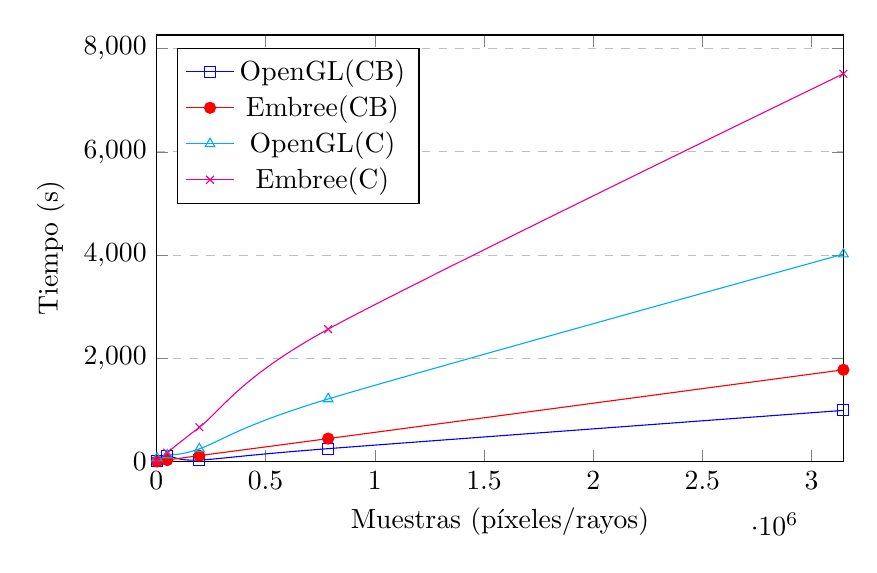
\begin{tikzpicture}
\begin{axis}[
xlabel={Muestras (píxeles/rayos)},
ylabel={Tiempo (s)},
xmin=0, xmax=3145728,
ymin=0,
width=.85\textwidth, height=7cm,
legend pos=north west,
ymajorgrids=true,
grid style=dashed,
]

\addplot[
smooth,
color=blue,
mark=square,
]
coordinates {
	(3072,7)(49512,105)(196608,31)(786432,251)(3145728,992)
};
\addplot[
smooth,
color=red,
mark=*,
]
coordinates {
	(3072,3)(49512,30)(196608,116)(786432,446)(3145728,1778)
};

\addplot[
smooth,
color=cyan,
mark=triangle,
]
coordinates {
	(3072,68)(49512,128)(196608,248)(786432,1213)(3145728,4018)
};

\addplot[
smooth,
color=magenta,
mark=x,
]
coordinates {
	(96,14)(49512,174)(196608,665)(786432,2565)(3145728,7511)
};

\legend{OpenGL(CB),Embree(CB),OpenGL(C), Embree(C)}

\end{axis}
\end{tikzpicture}
\caption{Comparación del rendimiento de los algoritmos en escenas exclusivamente difusas}
\label{plot:emglc1}
\end{figure}

Una de las consecuencias más interesantes a ser analizadas para detectar la cantidad de muestras óptimas a considerar es la calidad de la imagen final, y qué tan pronunciadas son las diferencias en la iluminación entre los parches, es decir, en qué medida difiere la radiosidad entre parches. Para este caso, se pudo observar (véase la Figura \ref{img:difres}) que si bien las resoluciones más bajas consumen menor cantidad de recursos los resultados tienen una calidad sustancialmente menor. Considerando que el modelo generalmente es utilizado para el cálculo de iluminación en una etapa de pre-procesado (fuera de línea), es recomendable evitar el uso de factores de muestreo tan bajos. Esto se ve acentuado en el análisis de la matriz de factores de forma, según las métricas establecidas en \ref{metricasestablecidas} se pudo comprobar que máximo error promedio apreciado (medida que se ha denominado $Ep$) fue de $0,05$ y $0,04$ utilizando $786.432$ muestras para los métodos del hemi-cubo y el hemisferio mientras que el uso de $3.072$ muestras generó errores del entorno de los $0,14$ y $0,06$ respectivamente. Estos se ven aún más acentuados al realizar el cálculo de la radiosidad para cada parche.

\begin{figure}[htbp]
	\centering
	\begin{subfigure}{0.45\textwidth}
		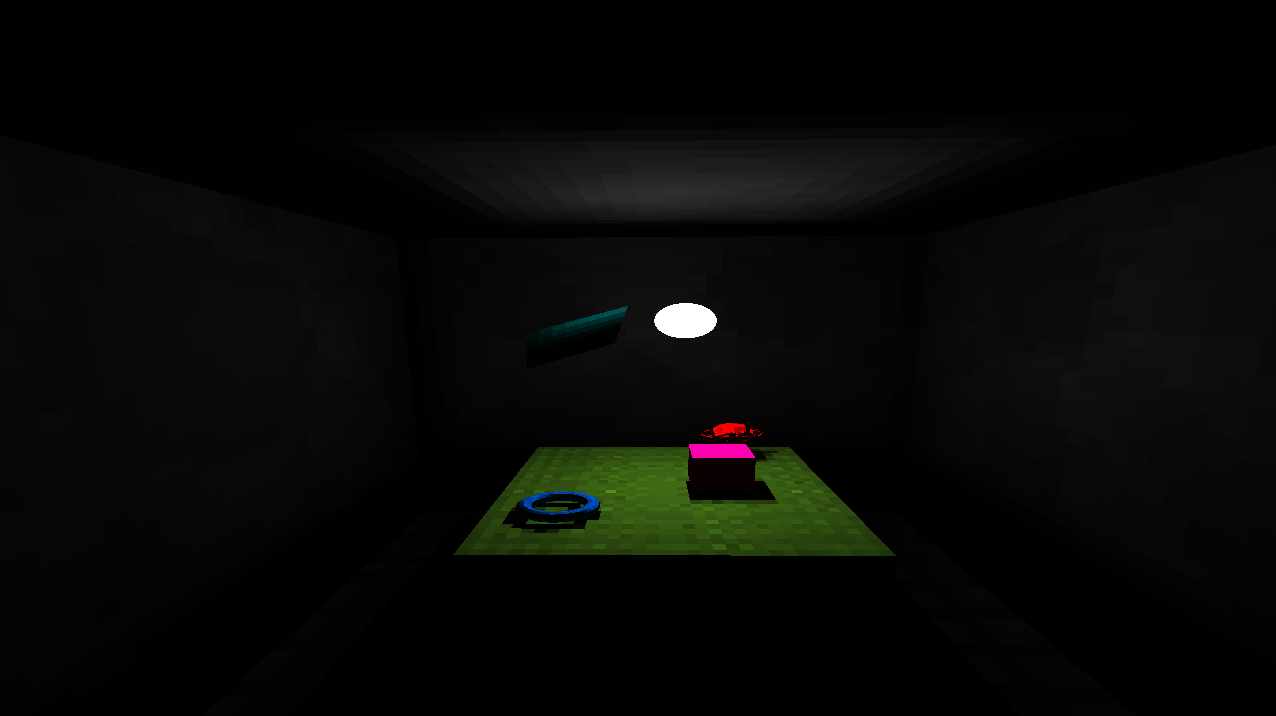
\includegraphics[width=1\linewidth]{assets/32sgl}
		\caption{OpenGL - 32 píxeles por cara}
	\end{subfigure}
	\begin{subfigure}{0.45\textwidth}
		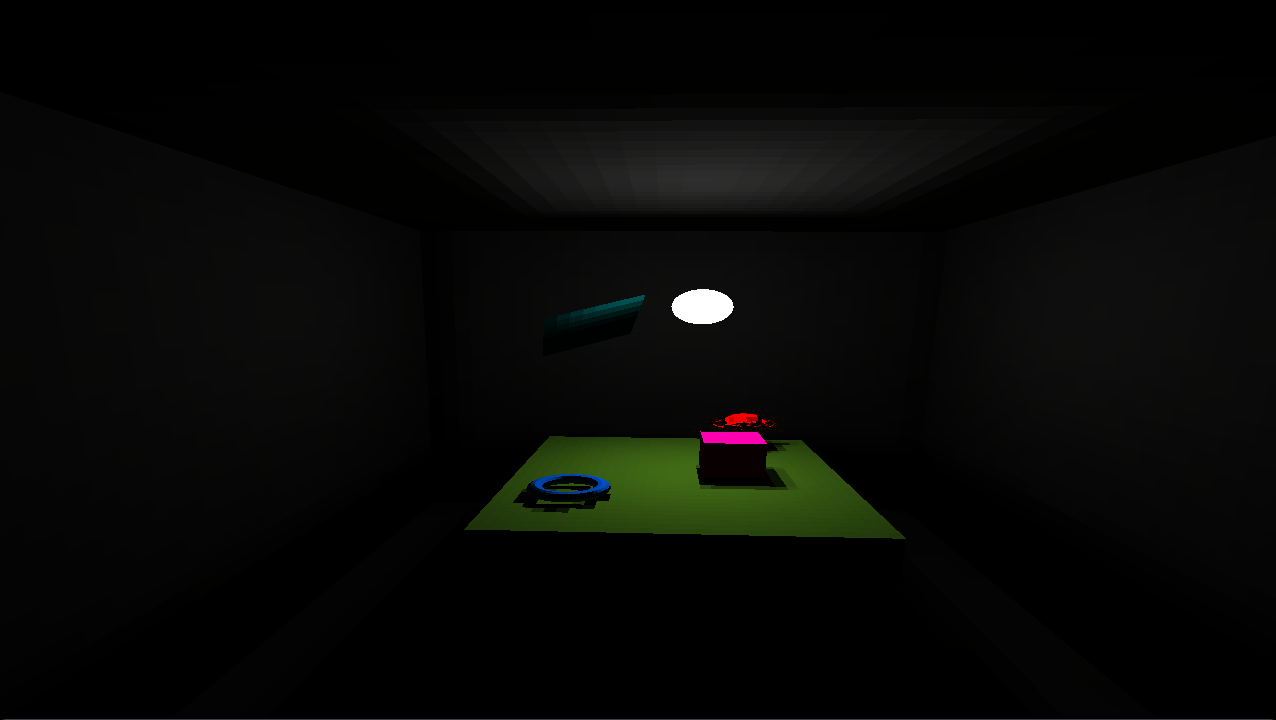
\includegraphics[width=1\linewidth]{assets/512sgl}
		\caption{OpenGL - 512 píxeles por cara}
	\end{subfigure}
	\begin{subfigure}{0.45\textwidth}
		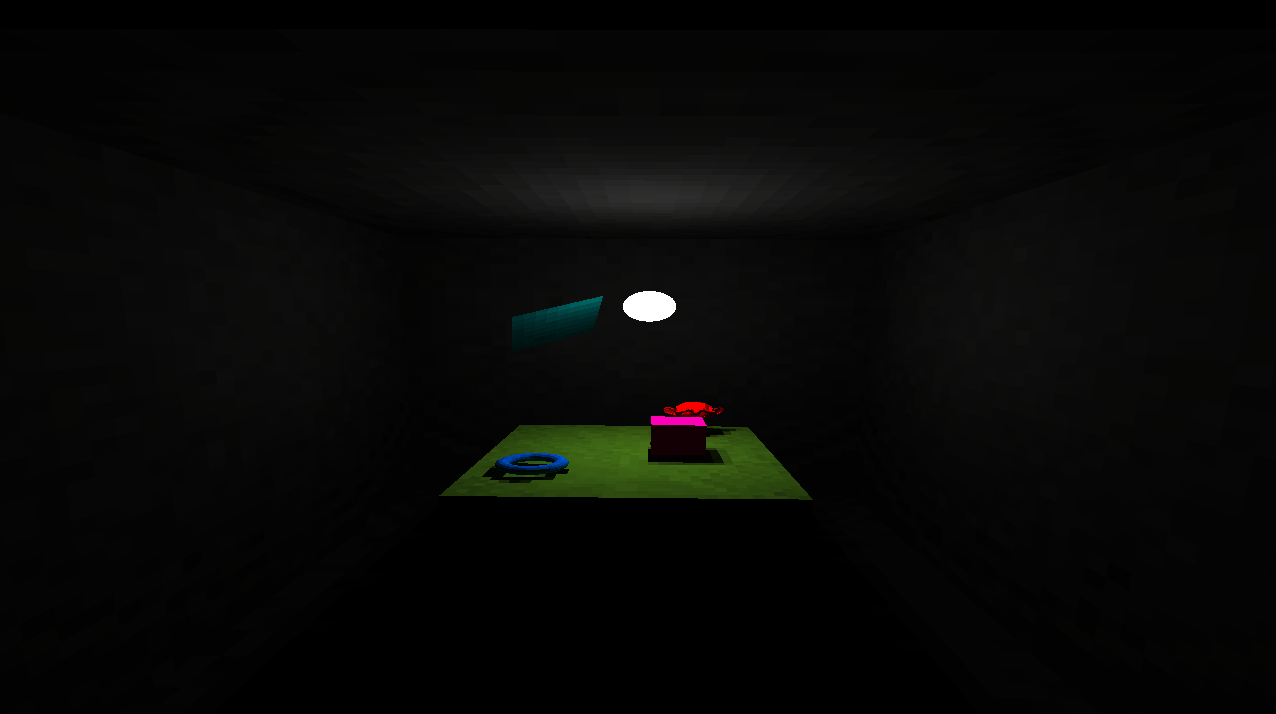
\includegraphics[width=1\linewidth]{assets/32srt}
		\caption{Embree - 3072 rayos}
	\end{subfigure}
	\begin{subfigure}{0.45\textwidth}
		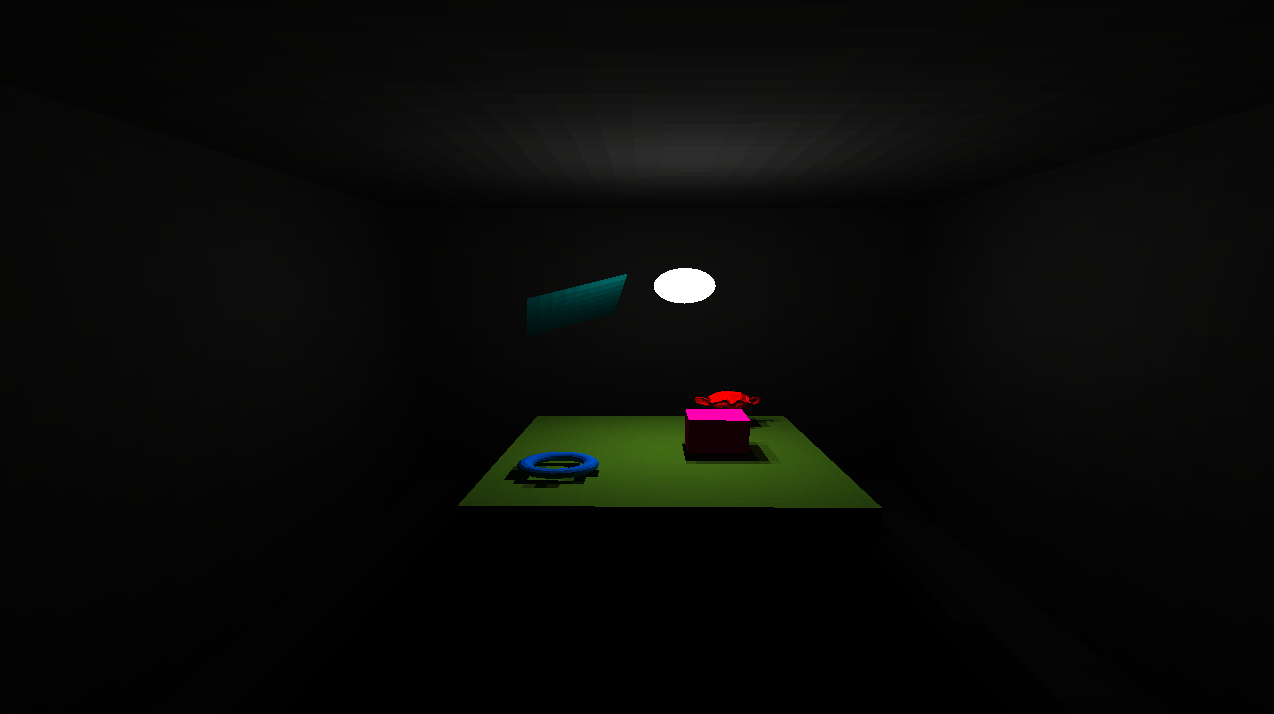
\includegraphics[width=1\linewidth]{assets/512srt}
		\caption{Embree - 786432 rayos}
	\end{subfigure}
	\caption{Diferencias visuales ajustando la cantidad de muestras}
	\label{img:difres}
\end{figure}

\subsubsection{Caso de prueba II (Reflexión Difusa + Especular)}

En este caso, se observa en la tabla \ref{tab:caso2} que el mejor rendimiento se obtiene utilizando el método híbrido, esto se debe a los hilos que ejecutan los cálculos correspondientes al rebote especular (utilizando traza de rayos) son ejecutados en la CPU mientras la GPU procesa hemi-cubos. Esta observación se ve respaldada por el hecho de que, en promedio se observó una ocupación rondando en los entornos de 100\% de la CPU y 35\% GPU en el método híbrido, 75\% de la CPU y 30\% GPU en el método utilizando OpenGL y 99\% en la implementación que solo utiliza traza de rayos. 

\begin{table}[htbp!]
	\centering
	\begin{tabular}{|l|l|l|l|l||l|l|l|}
		\hline
		\multicolumn{2}{|c|}{\multirow{2}{*}{\textbf{Muestras}}} & \multicolumn{6}{c|}{\textbf{Tiempo de ejecución (s)}}                                                                                  \\ \cline{3-8} 
		\multicolumn{2}{|c|}{}                   & \multicolumn{3}{c||}{\textit{Cornell Box}}                 & \multicolumn{3}{c|}{\textit{Calle}}                      \\ \cline{1-8}
		\multicolumn{1}{|c|}{OpenGL} &\multicolumn{1}{c|}{Embree} & \multicolumn{1}{c|}{GL-D+S} & \multicolumn{1}{c|}{E-D+S} & \multicolumn{1}{c||}{Híb} & GL-D+S                 & E-D+S & Híb \\ \hline
		\textbf{32x32x3 - 32}                                &
		\textbf{3072x3 - 32}                                & 25                         & 53                          & \textbf{21}                           & 2563                   & 1221   & \textbf{943}     \\ \hline
		\textbf{256x256x3 - 32}                                &
		\textbf{196608 - 32}                               & 93                         & 134                         & \textbf{84}                          & \textbf{1054}                   & 2512   & 1643    \\ \hline
		\textbf{512x512x3 - 64} &\textbf{786432 - 64}                              & 304                        & 486                         & \textbf{228}                          & \multicolumn{1}{c|}{-} & 5342   & \textbf{4725}    \\ \hline
	\end{tabular}
	\caption{Resultados obtenidos en el segundo caso de prueba. Notación: GL, E, Híb corresponden a OpenGL, Embree e Híbrido. La notación 'D+S' indica que se utilizaron reflexiones difusas y especulares. Los valores de muestras a la derecha indican la resolución de los espejos. '-' indica casos de prueba que tomaron tiempos excesivos.}
	\label{tab:caso2}
\end{table}

El paralelismo de las implementaciones basadas en la GPU garantiza el mejor rendimiento, sin embargo, se pudo notar que el uso exclusivo de traza de rayos provee hasta 800 veces menor error máximo que los otros algoritmos implementados. En \textit{Cornell Box}, con 786.432 muestras se notó una diferencia de error máxima $Ep$ de $0,0080$ con el método híbrido y $0,0055$ utilizando el método de dibujado de portales, en comparación con el método de traza de rayos que logró un error de $0,1 \times 10^{-3}$.

\begin{table}[htbp!]
	\centering
	\begin{tabular}{|l|l|l|l|l|}
		\hline
		\multicolumn{2}{|c|}{\multirow{2}{*}{\textbf{Muestras}}} & \multicolumn{3}{c|}{\textbf{Error relativo (normalizado)}}\\ \cline{3-5} 
		\multicolumn{2}{|c|}{}                   & \multicolumn{3}{c|}{\textit{Cornell Box}}                                \\ \cline{1-5}
		\multicolumn{1}{|c|}{OpenGL} &\multicolumn{1}{c|}{Embree} & \multicolumn{1}{c|}{GL-D+S} & \multicolumn{1}{c|}{E-D+S} & \multicolumn{1}{c|}{Híb} \\ \hline
		\textbf{32x32x3 - 32}                                &
		\textbf{3072 - 32}                                & 0.0138                         & 0.000481                          & 0.0091                                \\ \hline
		\textbf{256x256x3 - 32}                               &
		\textbf{196608 - 32}                               & 0.0093                         & 0.000108                         & 0.0073                             \\ \hline
		\textbf{512x512x3 - 64} &\textbf{786432 - 64}                              & 0.0080                        & 0.000010                         & 0.0055                             \\ \hline
	\end{tabular}
	\caption{Resultados obtenidos en el segundo caso de prueba (Cornell Box).}
	\label{tab:caso2err}
\end{table}

Esto se debe a que tanto en el uso de dibujado de portales o el algoritmo híbrido se utilizan estimaciones de la dirección en la que rebotaría el rayo en el espejo considerado, lo que degrada la autenticidad final de los datos obtenidos, sobre todo en el dibujado de portales donde la granularidad de las muestras obtenidas es inferior (se toman muestras por área y no por rayo). Por lo tanto, incluso si el método de traza de rayos posee un tiempo de ejecución un tanto mayor (que se debe mayormente al hecho de que se ejecuta únicamente en la CPU) se observa una calidad de datos de órdenes de magnitud superior a la de los otros métodos.

\begin{figure}[htpb!]
	\centering
	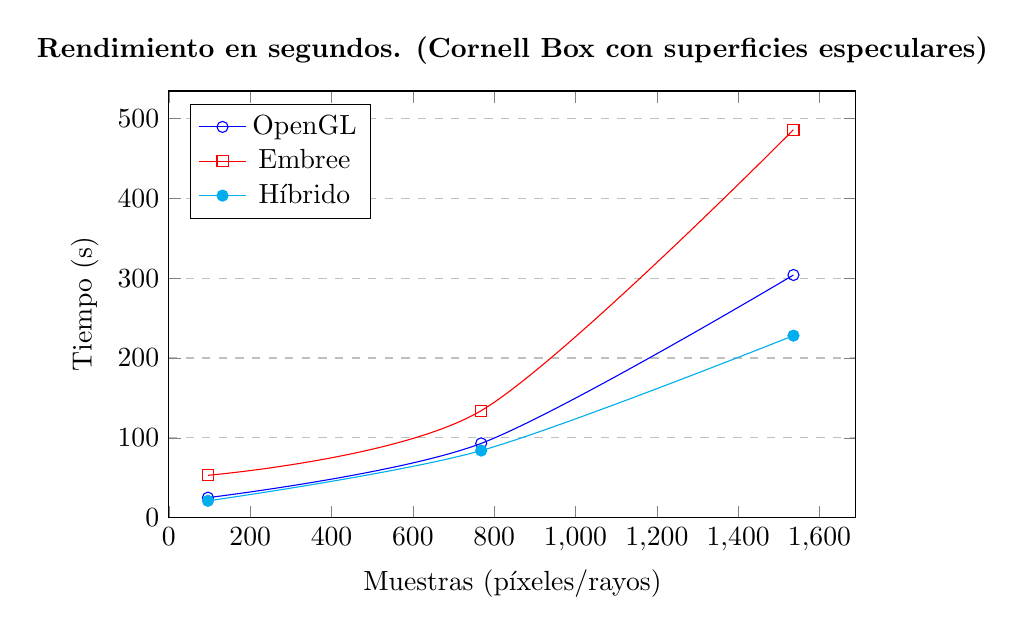
\begin{tikzpicture}
	\label{plot:emglc2}
	\begin{axis}[
	title={\textbf{Rendimiento en segundos. (Cornell Box con superficies especulares)}},
	xlabel={Muestras (píxeles/rayos)},
	ylabel={Tiempo (s)},
	xmin=0,
	ymin=0,
	width=.85\textwidth, height=7cm,
	legend pos=north west,
	ymajorgrids=true,
	grid style=dashed,
	]
	
	\addplot[
	smooth,
	color=blue,
	mark=o,
	]
	coordinates {
		(96,25)(768,93)(1536,304)
	};
	\addplot[
	smooth,
	color=red,
	mark=square,
	]
	coordinates {
		(96,53)(768,134)(1536,486)
	};
	
	\addplot[
	smooth,
	color=cyan,
	mark=*,
	]
	coordinates {
		(96,21)(768,84)(1536,228)
	};
	
	
	\legend{OpenGL,Embree,Híbrido}
	
	\end{axis}
	\end{tikzpicture}
	\caption{Rendimiento en segundos, considerando superficies especulares}
\end{figure}


\begin{figure}[htbp!]
	\centering
	\begin{subfigure}{0.5\textwidth}
		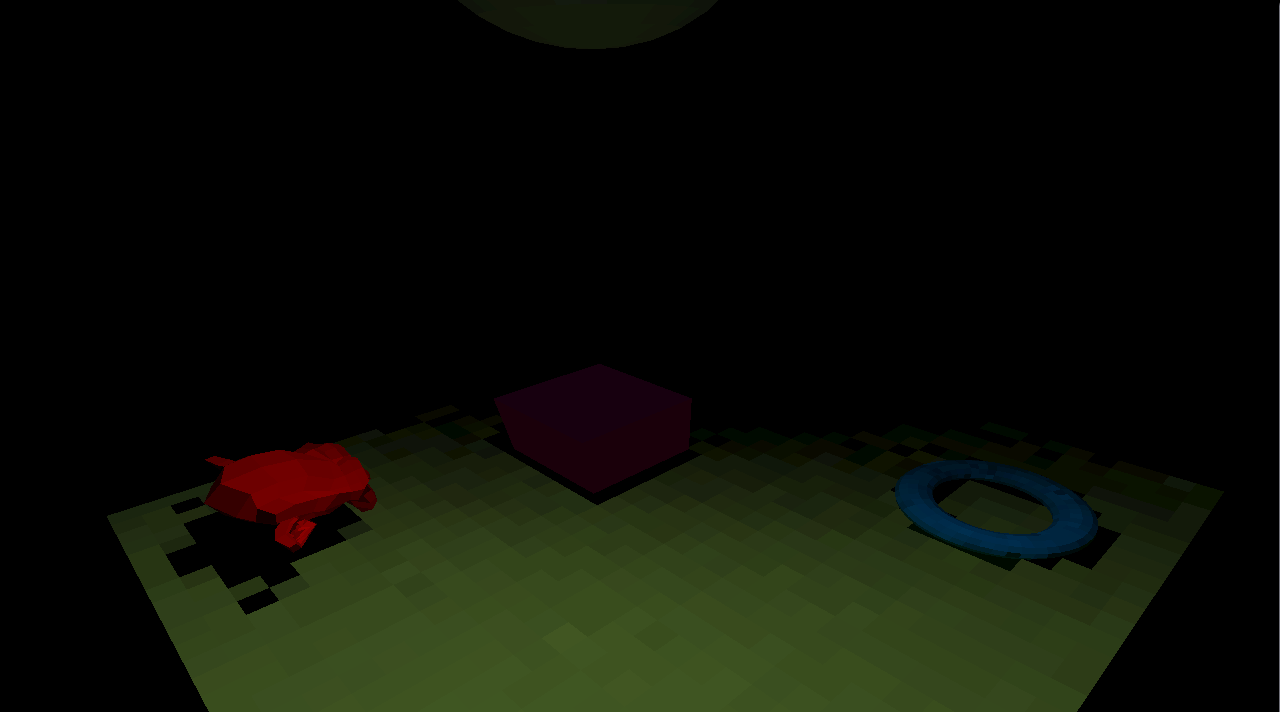
\includegraphics[width=1\linewidth]{assets/cornellesp2}
		\caption{OpenGL-D+S}
	\end{subfigure}
	\begin{subfigure}{0.5\textwidth}
		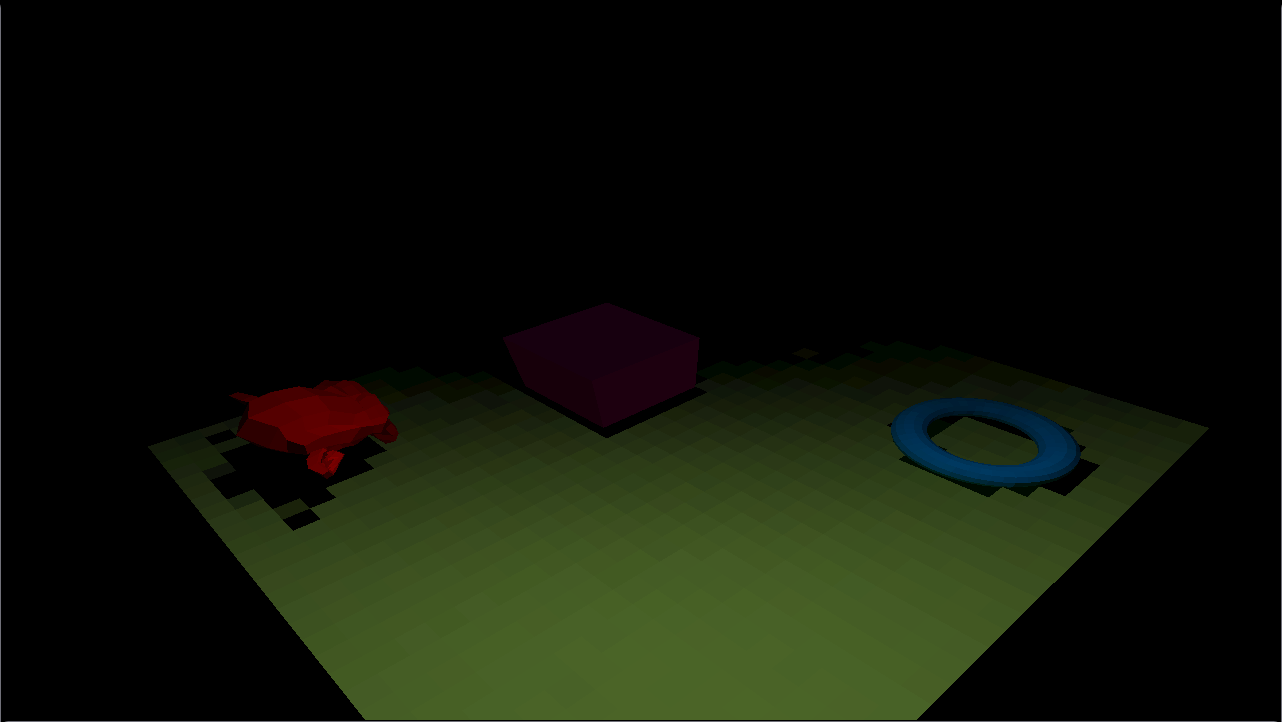
\includegraphics[width=1\linewidth]{assets/cornellespembree}
		\caption{Embree-D+S}
	\end{subfigure}
	\begin{subfigure}{0.5\textwidth}
		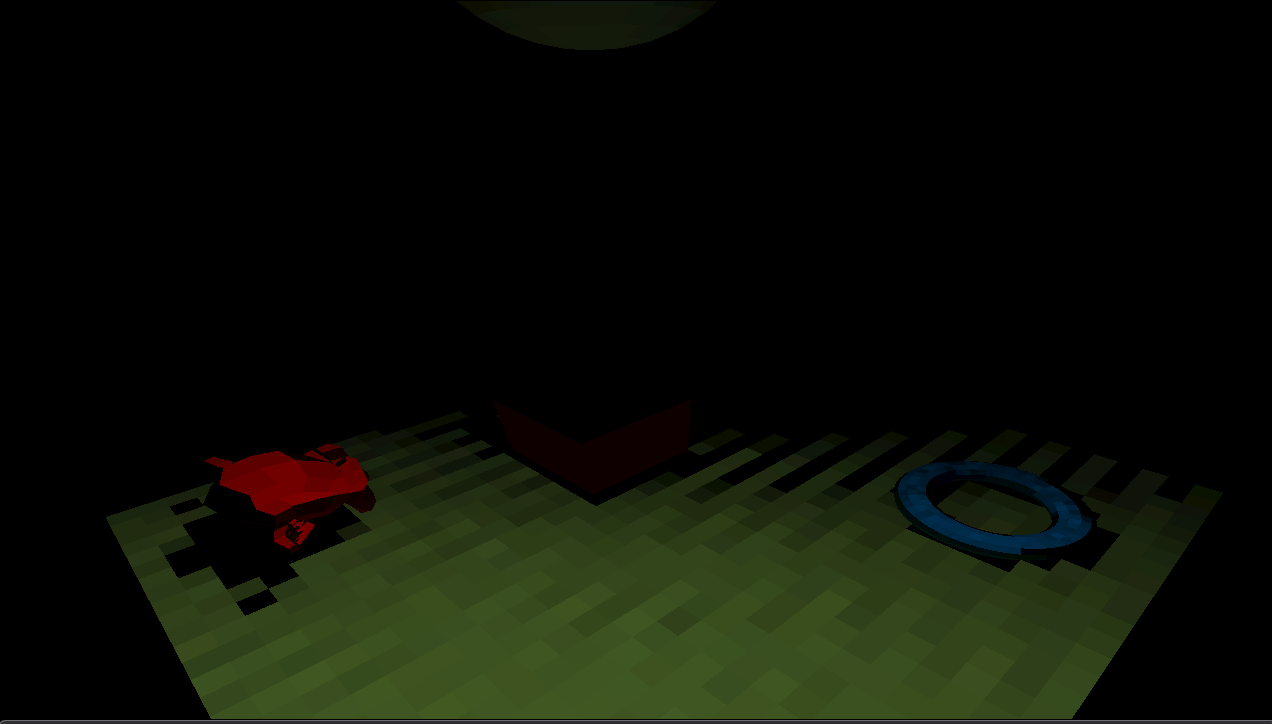
\includegraphics[width=1\linewidth]{assets/caso3esp}
		\caption{Híbrido}
	\end{subfigure}	
	\caption{Diferencias visualizadas utilizando las distintas implementaciones de cálculo de factores de forma extendido. 1536 muestras iniciales y 64 para rebotes especulares.}
	\label{img:difres2}
\end{figure}

Con el objetivo de cuantificar los datos de error observado se analizó el error promedio en el vector de radiosidad final (comparado a una muestra utilizando exclusivamente trazado de rayos con 786.432 muestras para el hemisferio) y se constató que, tal como se había supuesto, el método es significativamente menos propenso a generar errores como se ve en la Figura \ref{img:difres2}.

\begin{figure}[htbp!]
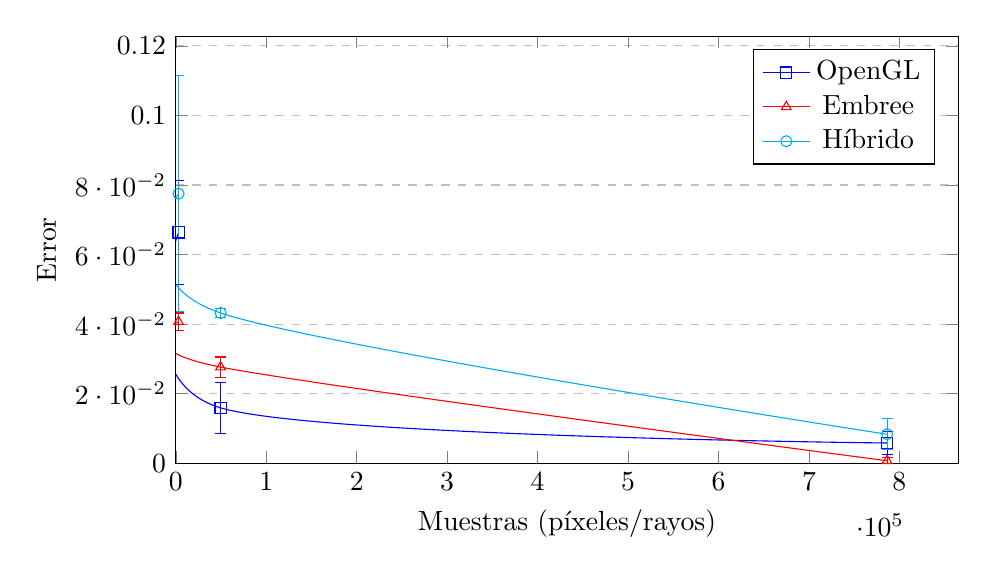
\begin{tikzpicture}
\begin{axis}[
xlabel={Muestras (píxeles/rayos)},
ylabel={Error},
xmin=0,
ymin=0,
width=.95\textwidth, height=7cm,
legend pos=north east,
ymajorgrids=true,
grid style=dashed,
]

\addplot[
smooth,
color=blue,
mark=square,
mark=square,error bars/.cd, y dir=both,y explicit
]
coordinates {
	(3072,0.06634) +- (0, 0.015)
	(49512,0.01593) +- (0, 0.0074)
	(786432,0.00582) +- (0, 0.0034)
};
\addplot[
smooth,
color=red,
mark=triangle,
mark=triangle,error bars/.cd, y dir=both,y explicit
]
coordinates {
	(3072,0.0406985) +- (0, 0.0025)
	(49512,0.02765) +- (0, 0.0029)
	(786432,0.000712) +- (0, 0.0009)
};

\addplot[
smooth,
color=cyan,
mark=* ,
mark=o,error bars/.cd, y dir=both,y explicit
]
coordinates {
	(3072,0.0775)  +- (0, 0.034)
	(49512,0.0432)  +- (0, 0.0014)
	(786432,0.008324)  +- (0, 0.0045)
};


\legend{OpenGL,Embree,Híbrido}

\end{axis}
\end{tikzpicture}
\caption{Error promedio observado en valor final de radiosidad en Híbrido. Los intervalos muestran el error máximo.}
\label{plot:errorcII}
\end{figure}

\subsubsection{Caso de prueba III (Conjunta)}

Esta prueba se construyó con el objetivo de comparar el rendimiento observado utilizando los algoritmos para el cálculo de factores de forma extendidos implementados. Es interesante comparar las diferencias en los tiempos de ejecución para una cantidad de muestras fijas, incluso si se han notado grandes discrepancias entre los resultados observados entre los métodos. Se ha puesto especial énfasis en las diferencias producidas al variar la cantidad de caras especulares de la escena, es decir, los parches cuyo coeficiente de reflexión es positivo. Las pruebas se realizaron con una cantidad de muestras fijas (256x256x3 para el hemi-cubo o 196.608 rayos para Embree y 4.096 muestras para el portal).

\begin{table}[htbp!]
	\centering
	\caption{Pruebas realizadas en \textit{Cornell Box} para identificar incidencia en la cantidad de caras especulares utilizadas en el tiempo de ejecución}
\begin{tabular}{|l|l|l|l|}
	\hline
	\multicolumn{1}{|c|}{\textbf{Parches especulares}} & \multicolumn{1}{c|}{OpenGL (s)} & \multicolumn{1}{c|}{Embree (s)} & \multicolumn{1}{c|}{Híbrido (s)} \\ \hline
	\textbf{0}                              & \textbf{38}                          & 126                         & -                            \\ \hline
	\textbf{16}                             & 41                          & 118                         & \textbf{39}                           \\ \hline
	\textbf{32}                             & 48                          & 120                         & \textbf{40}                           \\ \hline
	\textbf{64}                             & 68                          & 121                         & \textbf{43}                           \\ \hline
\end{tabular}
	\label{tab:caso3}
\end{table}

En la Tabla \ref{tab:caso3} puede observarse cómo la traza de rayos supera en dos veces el tiempo a los otros algoritmos. Sin embargo, se ha de destacar (al igual que en las pruebas anteriores) que los resultados observados tendrían variaciones en caso de utilizarse resoluciones mayores para el dibujado de portales. En cuyo caso, los tiempos entre los casos de prueba serían más afines, aunque se conseguirían resultados peores dada las aproximaciones realizadas en el dibujado de portales. Esto se demuestra al emparejar la cantidad de muestras tomadas por el portal con las de cada cara del hemi-cubo (256); en este caso los tiempos de ejecución para $62$ parches especulares es de 150 segundos. Por lo tanto, si bien existe un tiempo de ejecución mayor la estabilidad (en tiempo de ejecución) y la calidad de los datos obtenidos hacen que el método de traza de rayos sea superior a las otras dos propuestas.

\begin{figure}[htbp!]
	\centering
	\begin{subfigure}{0.47\textwidth}
		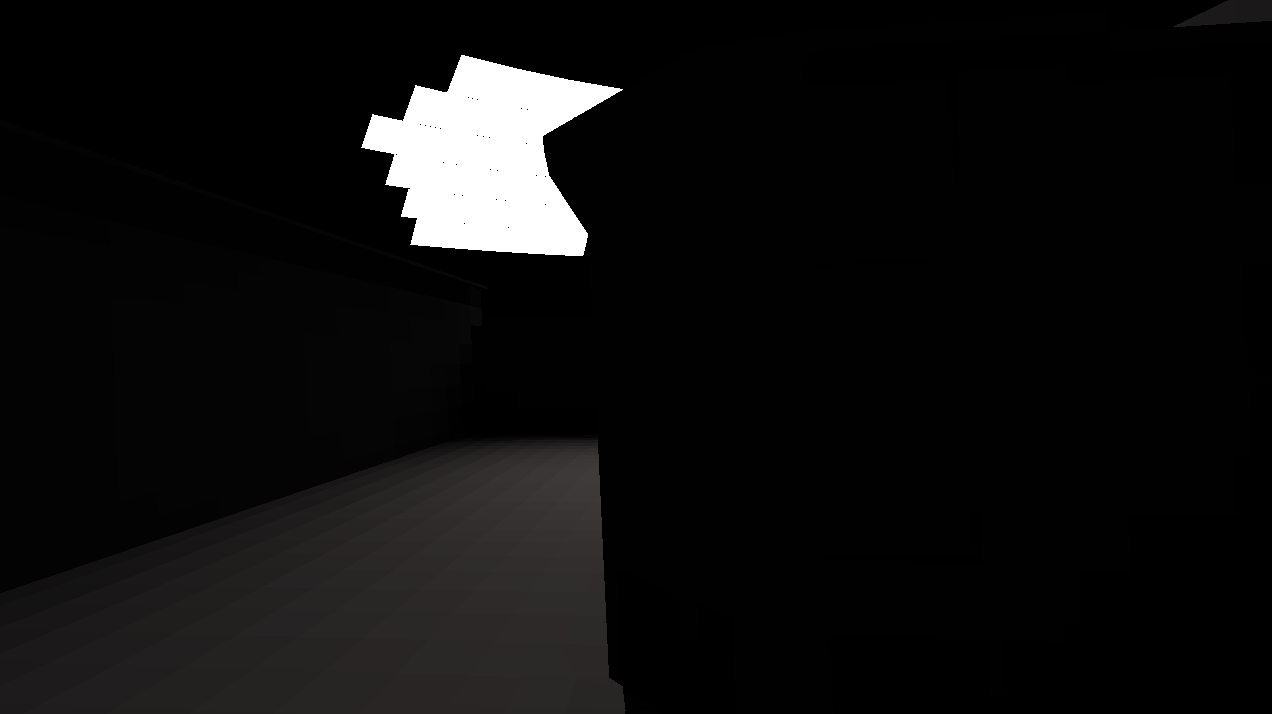
\includegraphics[width=1\linewidth]{assets/streete}
		\caption{Extensión desactivada}
	\end{subfigure}
	\begin{subfigure}{0.47\textwidth}
		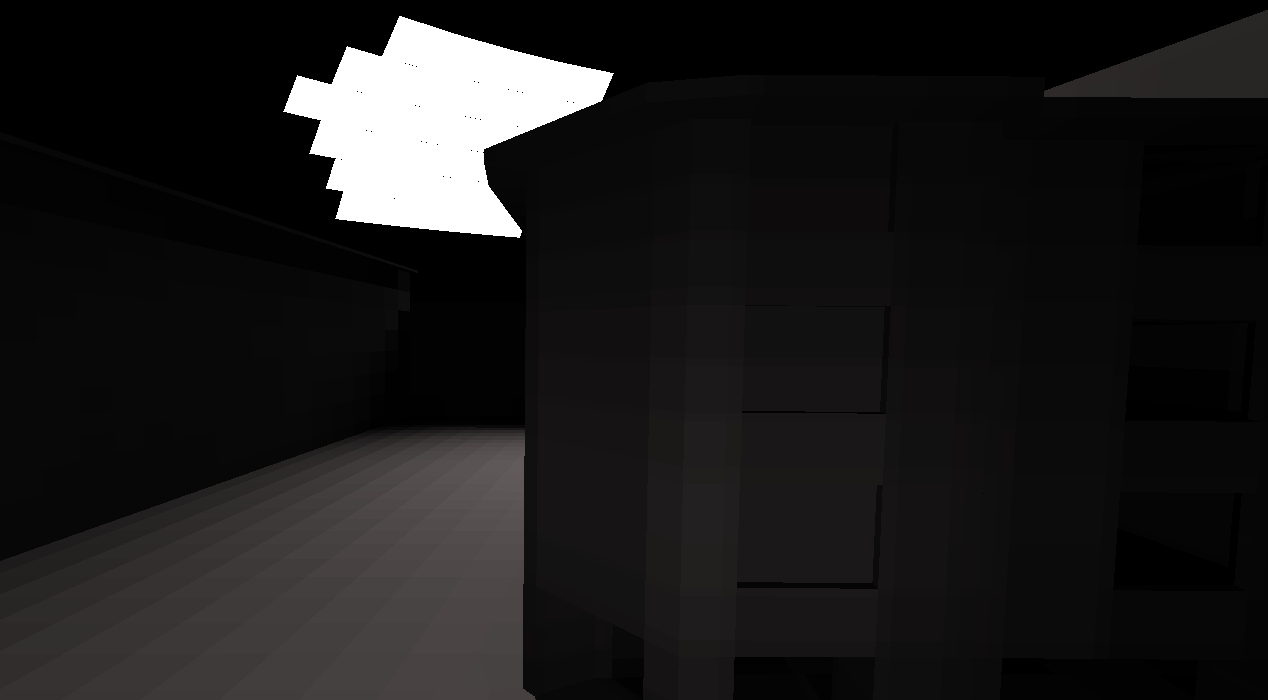
\includegraphics[width=1\linewidth]{assets/streets}
		\caption{Extensión activada}
	\end{subfigure}
	\caption{Diferencias observadas activando y desactivando extensiones}
	\label{img:difspecstreet}
\end{figure}

Adicionalmente, como se puede observar en la Figura \ref{img:difspecstreet}, las diferencias obtenidas en el valor final de la iluminación en cada parche pueden ser sutiles no obstante asemejan la simulación a escenarios reales con un costo despreciable en el tiempo de ejecución. En esta prueba en particular, se notó un aumento de aproximadamente 20 segundos (de 670 a 690). Donde en el primer caso se utilizó únicamente la iluminación difusa mientras que en segundo caso se activó la extensión utilizando trazado de rayos.

\subsubsection{Caso de prueba IV (Stress)}

Finalmente, con el objetivo de evaluar el impacto de contar con muchas superficies especulares se probó qué tanto tiempo adicional insume la carga impuesta al algoritmo del hemisferio (Embree) para considerar este tipo de superficie. Los resultados pueden observarse en la Figura \ref{plot:este}. Se notó una diferencia máxima de 3\% del tiempo de cálculo de los factores de forma al variar la cantidad de superficies especulares entre 0 y 1500 parches. Es por ello que se puede concluir que al utilizar algoritmos de traza de rayos no se detecta un impacto significativo en el tiempo de ejecución.

\begin{figure}[htbp!]
	\centering
	\resizebox{0.7\textwidth}{!}{
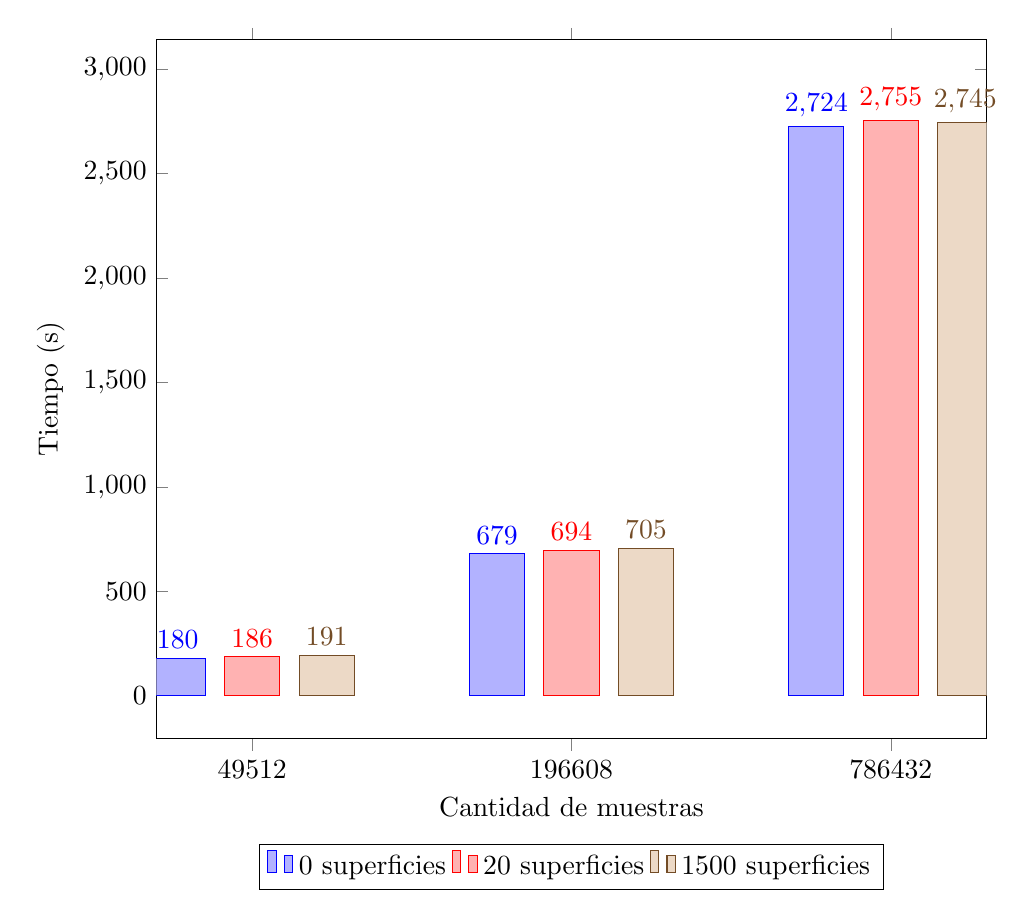
\begin{tikzpicture}

\begin{axis}[
ybar=7pt,
enlargelimits=0.15,
bar width=0.7cm,
legend style={at={(0.5,-0.15)},
	anchor=north,legend columns=-1},
ylabel={Tiempo (s)},
xlabel={Cantidad de muestras},
symbolic x coords={49512,196608,786432},
xtick=data,
nodes near coords,
nodes near coords align={vertical},
width=\linewidth
]
\addplot coordinates {(49512,180) (196608,679) (786432,2724)};
\addplot coordinates {(49512,186) (196608,694) (786432,2755)};
\addplot coordinates {(49512,191) (196608,705) (786432,2745)};
\legend{0 superficies, 20 superficies, 1500 superficies}
\end{axis}
\end{tikzpicture}}
\caption{Variación en el tiempo de ejecución en función de la cantidad de muestras y superficies especulares}
\label{plot:este}
\end{figure}


  \chapter{Conclusiones y trabajo futuro}
\label{ch:chap06}

\section{Conclusiones}
\label{sec:conclusiones}

\section{Trabajo futuro}
\label{sec:futuro}
  \afterpage{\blankpage}

  \listoffigures	        
  \listoftables	         	
  
  \backmatter 
  
  \apenarabicnumbering
  \apenmatter
  	\afterpage{\blankpage}

  Apéndice

  \bibliography{bibliography} 
  \bibend

  
\end{document}

% ===== FIN DEL DOCUMENTO =====

